\documentclass[11pt,a4paper]{article}
\usepackage[T1]{fontenc}\usepackage[utf8]{inputenc}\usepackage{lmodern}
\usepackage{microtype}\usepackage{geometry}\geometry{margin=1in}
\usepackage{amsmath,amssymb,amsfonts,amsthm,mathtools}
\usepackage{graphicx,float,booktabs,array,multirow,enumitem,tabularx,longtable}
\usepackage[numbers,sort&compress]{natbib}
\usepackage[colorlinks=true,linkcolor=blue,citecolor=blue,urlcolor=blue]{hyperref}
\usepackage{caption,xcolor,siunitx,listings}
\emergencystretch=2em

\lstset{basicstyle=\ttfamily\small,breaklines=true,frame=single,
        columns=fullflexible,backgroundcolor=\color{gray!6}}

\newtheorem{theorem}{Theorem}\newtheorem{lemma}{Lemma}
\newtheorem{corollary}{Corollary}\newtheorem{proposition}{Proposition}
\newtheorem{definition}{Definition}\newtheorem{assumption}{Assumption}
\newtheorem{remark}{Remark}

\DeclareMathOperator{\Tr}{Tr}\DeclareMathOperator{\rank}{rank}
\newcommand{\cD}{\mathcal{D}}\newcommand{\cH}{\mathcal{H}}
\newcommand{\cN}{\mathcal{N}}\newcommand{\cR}{\mathcal{R}}
\newcommand{\cU}{\mathcal{U}}
\newcommand{\cC}{\mathcal{C}}
\newcommand{\norm}[1]{\left\lVert #1\right\rVert}
\newcommand{\ket}[1]{\lvert #1\rangle}
\newcommand{\proj}[1]{\lvert #1\rangle\!\langle #1\rvert}

\title{Certified Adversarial Risk Bounds for Quantum Error-Correcting Memories:\\
Injection-Budget Certification with Simultaneous Intervals and\\
Reproducible Three-Code Bivariate-Bicycle Benchmarks}

\author{Saleh H.\ AlDaajeh$^{1}$, [AUTHOR 2: name]$^{2}$, [AUTHOR 3: name]$^{3}$\\[2pt]
[AUTHOR 4: name]$^{4}$, [AUTHOR 5: name]$^{5}$\\[4pt]
\small $^{1}$Independent Researcher, Information Systems and Security; \texttt{S.aldaajeh@gmail.com}\\
\small ORCID: \href{https://orcid.org/0000-0001-7810-9290}{0000-0001-7810-9290}\\
\small $^{2}$[AUTHOR 2: affiliation, email]\\
\small $^{3}$[AUTHOR 3: affiliation, email]\\
\small $^{4}$[AUTHOR 4: affiliation, email]\\
\small $^{5}$[AUTHOR 5: affiliation, email]\\[4pt]
\small Archive: prepared for Zenodo deposition; doi:10.5281/zenodo.20588043 (published June 2026)\\[2pt]
\small QEC Emulator v1.2.4~\cite{AlDaajeh2026emulator}
(ldpc~2.4.1, pymatching~2.2.2, stim~1.16.0, numpy~2.5.2)}
\date{\today}

\begin{document}
\maketitle

%%-----------------------------------------------------------
\begin{abstract}
%%-----------------------------------------------------------
We certify \emph{adversarial risk bounds} for quantum error-correcting
memories: for a fixed implementation (code $+$ schedule $+$ decoder)
and a bounded-weight fault-injection adversary, the operational risk
$\lambda_{\mathcal{M}}(W)=\max_{|F|\le W}\Pr[\text{logical failure}\mid
F]$ is estimated on device and reported as simultaneous intervals
$[L_W,U_W]$ at joint $\ge95\%$ confidence (Bonferroni-simultaneous;
exact Clopper--Pearson at zero counts), with honest $U_W=1$ wherever
the weight region is not exhausted.
The theory pairs two acknowledged background tools---a channel-game
minimax saddle point and a Knill--Laflamme fidelity floor---with new
elements: a spacetime-budget correctability theorem with sharpness and
device-aware composition, extended to CSS memories, plus a corrected
Pauli-channel bridge from either-sector logical failure rates to
diamond-norm bounds. Experiments use the open-source QEC
Emulator v1.2.4 with deterministic seeds and SHA-256 provenance.
Across three bivariate-bicycle codes: an exhaustive BB[[72,12,6]]
certificate ($d=6$ exactly; published witnesses, independent checker);
benchmarks in which BP+OSD lies far below two graphified matching
baselines (risk ratios $67.8\times$ to $>$134{,}000$\times$, joint
$\ge95\%$); a pinned seven-decoder paired grid on 70{,}000
bit-identical instances (BP augmentation closes the gap to BP+OSD;
bare symmetry matching is non-viable); circuit-level corroboration on
one pinned operating point, where Relay-BP separates from BP+OSD (the
two are statistically tied at code capacity); and a five-decoder
re-analysis of the released Kunlun $[[18,4,4]]$ detector model. On
ibm\_marrakesh, calibration-informed placement lowered logical error in
all four configurations ($p=0.042$); an injection test with protocols,
masks, and decision rules hash-pinned before submission
confirmed the distance cliff ($92$--$96\%$ collapse) and the
device-aware composed bound on every tested arm, replicating across
calibration cycles, devices, and distance~7; stochastic cells meet
mask-conditioned thresholds in both campaigns (the conditioning
estimand was corrected retrospectively in campaign~1 and pinned before
submission for the consolidation; chronology disclosed in
Appendix~\ref{app:chronology}).
These results assemble into a scoped integrity-evidence profile with an
explicit threat model; syndrome-only monitoring is proved insufficient.

\end{abstract}

\noindent\textbf{Keywords:} qLDPC; bivariate-bicycle codes; adversarial
channels; minimax; entanglement fidelity; BP+OSD; MWPM; DEM decomposition;
reproducible benchmarks; open-source scientific software.

%%-----------------------------------------------------------
\section{Introduction}
%%-----------------------------------------------------------

Fault-tolerant quantum computing and post-quantum cryptography are
strategically coupled~\cite{Shor1997,NISTFIPS203,NISTFIPS204,NISTFIPS205}.
The bivariate-bicycle (BB) code family~\cite{Bravyi2024} provides a
high-rate, weight-six qLDPC substrate suitable for both defensive
deployment and adversarial analysis.

\paragraph{Specific gap.}
Prior BB benchmarks~\cite{Bravyi2024,ShawRengaswamy2026} use BP+OSD;
this paper adds a transparent graphified DEM-MWPM reference baseline compatible with PyMatching-style graphlike inputs, together with a three-code same-protocol reproducibility archive with SHA-256 manifests.
We fill these gaps for the tested implementations and find that the two graphified baselines perform substantially worse than BP+OSD under this protocol.

\subsection{What this paper claims (precise)}

\begin{enumerate}[leftmargin=1.6em,label=(\roman*)]
  \item \textbf{Certified adversarial risk bounds as the central object.}
    The fixed-implementation adversarial risk
    $\lambda_{\mathcal{M}}(W)$ (Definition~\ref{def:acevalue}), reported
    as simultaneous intervals $[L_W,U_W]$ with honest $U_W=1$ outside
    tested regions (Remarks~\ref{rem:central-estimand},
    \ref{rem:intervals}); a four-category decoder endpoint separating
    wrong-logical corrections from invalid ones
    (Definition~\ref{def:endpoint}).
  \item Background (acknowledged standard, not a contribution): minimax
    saddle point via Sion's theorem; Knill--Laflamme fidelity floor.
  \item Architectural scaling lemma on logical-operator weight.
  \item QEC Emulator v1.2.4 --- open-source software infrastructure for all
    experiments, with five independently extensible layers and SHA-256 provenance.
  \item BB72 certificate: $d=6$ exact, $t=2$ exhaustive, SHA-256 matrix pins.
  \item Three-code single-round BP+OSD vs DEM-MWPM, 10{,}000 trials, CIs,
    with a $10^{6}$-trial rare-event refinement at $p\in\{0.002,0.004\}$.
  \item Three-code repeated-cycle BP+OSD ($d$~rounds), 2{,}000--500 trials, CIs,
    plus 4{,}000--20{,}000-trial adaptive extensions.
  \item Three-code finite-size evidence (sub-threshold ordering, not formal FSS).
  \item Hardware ablation (simulation models only): SWAP routing, measurement noise, and gate-decoherence parameters materially affect the simulated CZ/MS gap; no real-hardware causal claim is made.
  \item UF-BFS provides a second graphified baseline; it also underperforms BP+OSD under the submitted protocol.
  \item Decoder-dependent ACE gap (Remark~\ref{rem:decoder-gap}; upgraded from
    proxy to bound under the Pauli approximation by
    Proposition~\ref{prop:bridge}).
  \item Injection-budget game: operational ACE value
    (Definition~\ref{def:acevalue}), spacetime-budget correctability theorem
    with sharpness construction (Theorem~\ref{thm:spacetime}), device-aware
    composition bound (Corollary~\ref{cor:stoch}).
  \item Device test of the theory layer on ibm\_marrakesh with
    protocols, masks, and decision rules hash-pinned before submission
    (Appendix~\ref{app:injection}, 312 arms, 180{,}000 shots): weight-$t$
    worst-case injections bounded, weight-$(t{+}1)$ collapse at
    $92$--$96\%$; all stochastic cells hold against mask-conditioned
    thresholds in both campaigns (campaign-1 conditioning estimand
    corrected retrospectively --- Appendix~\ref{app:chronology}); the
    device-aware composed bound holds on all tested arms.
  \item No asymptotic threshold; no IND-CPA.
\end{enumerate}

%%-----------------------------------------------------------
\section{Related work}
%%-----------------------------------------------------------

BB codes and their threshold~\cite{Bravyi2024};
networked BB codes~\cite{ShawRengaswamy2026};
BP+OSD~\cite{Roffe2020,ldpcPackage};
PyMatching/Sparse Blossom~\cite{Higgott2023,SparseBlossom2025};
Stim~\cite{Gidney2021};
qLDPC families~\cite{TillichZemor2014,PanteleevKalachev2022,LeverrierZemor2022};
FTQC overhead~\cite{Gottesman2014,FawziGrospellierLeverrier2018,
ChristandlFawziGoswami2025};
post-quantum standards~\cite{NISTFIPS203,NISTFIPS204,NISTFIPS205};
QKD~\cite{BennettBrassard1984,ShorPreskill2000,PortmannRenner2022};
formal verification~\cite{RandPaykinZdancewic2018,Hietala2021,
Bordg2021,Lewis2023}.

\paragraph{Decoder landscape, 2025--2026.}
Relay-BP, a BP variant with disordered memory strengths targeting real-time
circuit-level decoding~\cite{Muller2025relay} with an FPGA prototype on
$[[144,12,12]]$~\cite{Johnson2026relayfpga};
symmetry matching (\texttt{symatch}), which exploits the equivalence of BB
codes to toric-code copies~\cite{SahayBrown2026};
belief-matching hybrids that reweight matching graphs with BP
posteriors~\cite{Higgott2023belief};
trapping-set analyses of detector error
models~\cite{Pacenti2026trapping};
and the below-threshold $\Lambda$-ladder reporting standard of
Acharya et al.~\cite{Acharya2024lambda}.
On hardware, the Kunlun processor operated a $[[18,4,4]]$ BB code and
released its detector matrices openly~\cite{Wang2026kunlun}, and a
controlled study of defective components contrasted defect exclusion with
defect-aware decoding~\cite{Bartlett2026defect}.

\paragraph{Closest prior art.}
Table~\ref{tab:priorart} positions this work against the nine closest
sources. The strongest comparison is the Fail-fast framework
of~\cite{beverland2025failfast}: both works inject structure to probe
rare QEC failures, but the estimands differ --- fail-fast accelerates
\emph{nominal stochastic} rare-event estimation (importance-style
variance reduction under the device's own noise law), whereas we bound
\emph{worst-case adversarial} risk $\lambda_{\mathcal{M}}(W)$ over
fault-set placement with simultaneous $[L_W,U_W]$ intervals; the two
are complementary, and fail-fast sampling is a candidate accelerator
for our $U_W$ estimation at large $W$. The trapping-set analysis
of~\cite{Pacenti2026trapping} is closest in spirit on decoder failure
structure; it characterizes failure configurations of a
\emph{stochastic} DEM, while our injection-boundary study fixes the
code and varies an \emph{adversarial} weight budget, separating
wrong-logical corrections from residual-carrying invalid corrections
(four-category endpoint) --- a distinction the trapping-set frame does
not track.

\begin{table}[H]\centering\small
\caption{Closest prior art and differentiation. Scope abbreviations:
  nom.\ = nominal stochastic noise; adv.\ = adversarial placement.}
\label{tab:priorart}
\begin{tabular}{@{}p{0.30\columnwidth}p{0.30\columnwidth}p{0.34\columnwidth}@{}}
\toprule
source & contribution & relation to this work \\\midrule
Bravyi et al.\ \cite{Bravyi2024} & BB codes, thresholds, hardware memory & we reuse the code family; they do not treat adversarial injection \\
Roffe et al.\ \cite{Roffe2020} & BP+OSD decoder & our reference decoder; benchmarked, not introduced here \\
Sahay et al.\ \cite{SahayBrown2026} & symmetry matching for BB codes & pinned-comparator subject; bare form non-viable on this instance, BP-augmented tied with BP+OSD \\
M\"uller et al.\ \cite{Muller2025relay} & Relay-BP real-time BP & benchmarked; circuit-level outcome separates from the code-capacity tie \\
Beverland et al.\ \cite{beverland2025failfast} & fail-fast rare-event probing (nom.) & strongest comparison; accelerated nom.\ estimation vs our adv.\ worst-case bounds; complementary \\
Pacenti et al.\ \cite{Pacenti2026trapping} & DEM trapping sets & stochastic failure structure; no adversarial budget or endpoint decomposition \\
Kosut et al.\ \cite{kosut2008robust} & recovery optimization for a fixed channel & defender-side optimization; our $\lambda_{\mathcal{M}}(W)$ fixes the implementation \\
Huang et al.\ \cite{huang2019coherent} & coherent-error channel analysis & basis of our twirling residual, which we close analytically \\
Acharya et al.\ \cite{Acharya2024lambda} & below-threshold $\Lambda$ reporting & reporting standard we delimit our block-$\Lambda$ against (no matched protocol) \\
\bottomrule
\end{tabular}
\end{table}
Section~\ref{sec:comparator} positions the present work against these
families quantitatively.

%%-----------------------------------------------------------
\section{QEC Emulator: software infrastructure}
\label{sec:emulator}
%%-----------------------------------------------------------

All experiments in this paper are conducted using the QEC Emulator
v1.2.4~\cite{AlDaajeh2026emulator}, an open-source Python package
released under the MIT licence at
doi:10.5281/zenodo.20588043 (published June 2026).
This section describes the emulator's design, scientific contributions,
and its role as a reusable research platform.

\subsection{Design philosophy and architecture}

The emulator is organised as five independent layers
(Figure~\ref{fig:emulator-arch}), each with a single scientific
responsibility:

\begin{enumerate}[leftmargin=1.6em,label=\textbf{L\arabic*.}]
  \item \textbf{Code construction} (\texttt{codes.py}) ---
    BB code algebra over $\mathbb{F}_2$, SHA-256 matrix fingerprints.
  \item \textbf{Decoders} (\texttt{decoders.py}) ---
    LookupDecoder, BPOSDDecoder, MWPMDecoder; common abstract interface.
  \item \textbf{Noise models} (\texttt{noise.py}) ---
    four models from phenomenological to hardware noise-model simulation.
  \item \textbf{Benchmark runners} (\texttt{benchmark.py}) ---
    five runners covering all experimental protocols in this paper.
  \item \textbf{Provenance} (\texttt{provenance.py}) ---
    SHA-256 integrity seals, manifest export, QC checks.
\end{enumerate}

The layers are strictly decoupled: adding a new decoder, noise model,
or benchmark runner requires subclassing or implementing a single
interface without modifying any other layer.

\begin{figure}[H]
\centering
\begin{tabular}{|c|}
\hline
\textbf{L1.\ Code construction} \\
\texttt{BBCode(ell, m, a\_exp, b\_exp)} $\to$ $H_X, H_Z$ + SHA-256 pins \\
\hline
\textbf{L2.\ Decoders} \\
\texttt{LookupDecoder} $\mid$ \texttt{BPOSDDecoder} $\mid$ \texttt{MWPMDecoder} \\
\texttt{BaseDecoder}: \texttt{decode\_z(syn)} $\to$ correction mask \\
\hline
\textbf{L3.\ Noise models} \\
\texttt{PhenomenologicalModel} $\mid$ \texttt{RepeatedCycleModel} \\
\texttt{CircuitLevelModel} $\mid$ \texttt{HardwareModel(CZ|MS)} \\
\hline
\textbf{L4.\ Benchmark runners} \\
\texttt{run\_sweep} $\mid$ \texttt{run\_repeated\_cycle} $\mid$ \texttt{run\_threshold\_scan} \\
\texttt{run\_fixed\_weight} $\mid$ \texttt{run\_distance\_certificate} \\
\hline
\textbf{L5.\ Provenance} \\
\texttt{ProvenanceRecord}: SHA-256(code, decoder, $p$, seed, failures) \\
\texttt{ProvenanceLogger}: CSV/JSON export, \texttt{unresolved\_pairs()} QC check \\
\hline
\end{tabular}
\caption{Five-layer architecture of QEC Emulator v1.2.4.
  Each layer has a single scientific responsibility and is independently
  extensible.}
\label{fig:emulator-arch}
\end{figure}

\subsection{Code construction layer}

The \texttt{BBCode} dataclass constructs BB codes from generator polynomial
exponents over $\mathbb{F}_2[x,y]/(x^\ell-1,y^m-1)$.
Three named constructors are pinned to this paper's three code instances:

\begin{center}
\small
\begin{tabular}{@{}lllrrl@{}}
\toprule
Constructor & $(\ell,m)$ & Polynomials & $n$ & $k$ & $H_X$ SHA-256 prefix \\
\midrule
\texttt{BB72()}  & $(6,\,6)$   & $A=x^3+y+y^2$, $B=y^3+x+x^2$ & 72  & 12 & \texttt{7ab0973b...} \\
\texttt{BB144()} & $(12,\,6)$  & same polynomials              & 144 & 12 & \texttt{195d5586...} \\
\texttt{BB288()} & $(12,\,12)$ & $A=x^3+y^2+y^7$, $B=y^3+x+x^2$ & 288 & 12 & \texttt{c06e721e...} \\
\bottomrule
\end{tabular}
\end{center}

\noindent
The BB288 polynomial parameters follow Bravyi et al.\ Table~1~\cite{Bravyi2024}.
Every \texttt{BBCode} instance exposes \texttt{hx\_sha256()} and
\texttt{hz\_sha256()} methods returning the full 64-character SHA-256
digest of the respective matrix's byte representation.
The full digests are:

\begin{center}
\small\ttfamily
\begin{tabular}{@{}ll@{}}
\toprule
Code & $H_X$ SHA-256 \\
\midrule
BB72  & 7ab0973bfd02e399d69728d26e67dbfa0e95bbc6ad2c5cf8bf309d667244a5a8 \\
BB144 & 195d5586a406f0194b89649b6a2499ec2b481edb81c91293daf1745d8b806641 \\
BB288 & c06e721ec6ea114b60e0e6f7187324f6e150e229b8d008888e8a4cc3f4a324a2 \\
\bottomrule
\end{tabular}
\end{center}

\noindent
A reviewer can verify any data table in this paper by (i)~running
\texttt{pip install qec-emulator}, (ii)~instantiating the named
constructor, and (iii)~comparing \texttt{hx\_sha256()} against the
digest above.
This creates a tamper-evident chain from published number back to
exact matrix bytes.

\subsection{Decoder layer and key discoveries}
\label{ssec:decoder-layer}

Three decoder classes share a common abstract base interface
(\texttt{decode\_z}, \texttt{decode\_x}, \texttt{decode\_success}),
making them interchangeable in all benchmark runners.

\paragraph{\texttt{LookupDecoder}.}
Exact radius-$t$ syndrome lookup, self-contained with no external
dependencies.
For BB72 with certified $d=6$ and $t=2$, the lookup table covers
all $\sum_{w=0}^{2}\binom{72}{w}=2{,}629$ weight-$\le2$ patterns;
the \texttt{run\_fixed\_weight} runner confirms zero failures over
all patterns exhaustively.

\paragraph{\texttt{BPOSDDecoder}.}
Wraps the \texttt{ldpc} package v2 \texttt{BpOsdDecoder} class API
\cite{ldpcPackage}.
The legacy \texttt{bposd\_decoder} function (v1 API) causes a
segmentation fault on some inputs in \texttt{ldpc}$\,\ge\,$2.0 and
must not be used.
This is a non-obvious breaking change; the emulator explicitly uses the
v2 class API and documents the reason.
Default parameters: min-sum BP, scaling factor 0.625, OSD-CS order 7,
100 maximum iterations.
If \texttt{ldpc} is absent the class falls back to \texttt{LookupDecoder}
with \texttt{is\_fallback=True}, so provenance records are never silently
mislabelled.

\paragraph{\texttt{MWPMDecoder} and the DEM chain decomposition.}
This is an important implementation detail documented here.
PyMatching v2~\cite{Higgott2023} strictly rejects parity-check matrix
columns with weight $>2$ (raises \texttt{ValueError}).
BB codes have column weight three: each data qubit triggers exactly
three syndrome checks.
Therefore, loading $H_X$ directly into PyMatching v2 crashes.

The emulator implements the DEM chain decomposition: each weight-3
column $\{a,b,c\}$ is split into two binary edges $\{a,b\}$ and
$\{b,c\}$ via the \texttt{add\_edge()} API, discarding the $\{a,c\}$
correlation.
Additionally, BB syndrome graphs can contain odd-parity connected
components arising from logical operators, which prevent perfect
matching; high-weight ($100\times$ log-likelihood) global boundary
edges on every detector node resolve this.

The experimental consequence (Section~\ref{sec:benchmark}) is large but deliberately
limited: the tested DEM-chain MWPM reference baseline is $67.8\times$ to
$>$1{,}000$\times$ worse than BP+OSD across the tested BB code instances
(BB72 finite; BB144/BB288 infinite where BP+OSD achieves zero failures).
This should not be read as a theorem about all matching-family decoders.
It shows that the submitted chain graphification is a lossy, reproducible
reference baseline; any future MWPM-family comparison for BB codes must
state precisely how weight-3 hyperedges, correlations, and boundary effects
are represented.

\subsection{Noise model layer}

\paragraph{\texttt{PhenomenologicalModel}.}
Independent Bernoulli Pauli errors at rate $p$, ideal syndrome readout.
Used for all single-round decoder comparisons.

\paragraph{\texttt{RepeatedCycleModel}.}
The v1.2.4 protocol required for proper multi-round benchmarking.
$d$ syndrome rounds per trial: rounds $1,\ldots,d-1$ apply independent
Bernoulli errors at rate $p$ to both data qubits and measurement bits;
round $d$ is noiseless.
Returns differential detector syndrome arrays of length
$d\times n_{\mathrm{checks}}$ for space-time decoders.
This model is not equivalent to $d$ independent single-round trials:
cumulative data errors and measurement noise correlate across rounds
in a way that single-round simulation cannot capture.

\paragraph{\texttt{CircuitLevelModel}.}
Single-cycle Pauli propagation through the BB 432-CNOT schedule with
ancilla preparation faults ($p_{\mathrm{prep}}$), gate faults
($p_{\mathrm{gate}}$), idle data-qubit decoherence
($p_{\mathrm{idle}} = 0.05\,p_{\mathrm{gate}}$ by default), and noisy
syndrome measurement ($p_{\mathrm{meas}}$).

\paragraph{\texttt{HardwareModel}.}
Architecture-parameterised single-cycle simulation for two backends:
CZ (superconducting, $T_1=150\,\mu\text{s}$, SWAP routing) and
MS (trapped-ion, $T_1>1\,\text{s}$, all-to-all connectivity).
Device parameters match published characterisations.

\subsection{Benchmark runner layer}

Five runners implement the complete experimental protocols of this paper.

\texttt{run\_sweep}: single-round sweep across a $p$-grid; one
\texttt{ProvenanceRecord} per (p, batch) pair.

\texttt{run\_repeated\_cycle}: proper repeated-cycle benchmark.
For \texttt{decoder\_type='bposd'}, constructs the space-time extended
check matrix:
\begin{equation}
  H_{\mathrm{ext}}
  = \bigl[H_{\mathrm{space}}\;\big|\;H_{\mathrm{meas}}\bigr],
  \quad H_{\mathrm{space}} = I_d \otimes H_X,
  \label{eq:spacetime}
\end{equation}
where $H_{\mathrm{meas}}$ captures consecutive-round measurement-flip
detection.
For \texttt{decoder\_type='mwpm'}, builds a space-time matching graph
with per-round data-qubit edges and between-round measurement-flip edges.

\texttt{run\_threshold\_scan}: multi-code finite-size comparison.

\texttt{run\_fixed\_weight}: fixed-weight random-sampling decoder policy
test (not a code-capability test beyond the certified radius).

\texttt{run\_distance\_certificate}: meet-in-the-middle exhaustive
distance lower-bound enumeration.

\subsection{Provenance layer}

The provenance layer is the core scientific contribution of the emulator.
Every \texttt{ProvenanceRecord} stores 15 fields including the SHA-256 of
$H_X$, the SHA-256 of $H_Z$, the integer seed, the trial count, the raw
failure count, the Wilson 95\% upper confidence bound, the UTC timestamp,
the Python/NumPy version, and an integrity seal:

\begin{equation}
\begin{split}
  \texttt{result\_sha256}
  = \mathrm{SHA256}\!\bigl(&
    \mathrm{JSON\_sort}(\mathrm{code},\, \mathrm{decoder},\, p,\,
    n_{\mathrm{trials}},\, \mathrm{seed},\\
    &\mathrm{failures},\,
    \texttt{hx\_sha256},\, \texttt{hz\_sha256})
  \bigr).
\end{split}
  \label{eq:integrity-seal}
\end{equation}

Any change to the code matrix, seed, trial count, or failure count
produces a completely different digest, making undetected manipulation
cryptographically infeasible.
The \texttt{unresolved\_pairs()} method flags any two records sharing
an identical \texttt{(code, decoder, p, result\_sha256)} tuple ---
distinguishing genuine zero-failure runs from seed collisions or
copy-paste errors.

\subsection{Open-source design and research extensibility}

QEC Emulator is released under the MIT licence and is explicitly
designed as a platform for further research.
Four extension points require no modification to the core package:

\begin{enumerate}[leftmargin=1.6em]
  \item \textbf{New BB code instance}: \texttt{BBCode(ell, m, a\_exp, b\_exp)}.
  \item \textbf{New CSS code}: override \texttt{hx} and \texttt{hz} in
    a \texttt{BBCode} subclass.
  \item \textbf{New decoder}: subclass \texttt{BaseDecoder} and implement
    \texttt{decode\_z} and \texttt{decode\_x}.
  \item \textbf{New noise model}: implement the four-return-value callable
    \texttt{(code, p, rng) $\to$ (z\_mask, x\_mask, syn\_z, syn\_x)}.
\end{enumerate}

Directions for academic extension include:
threshold analysis with $\ge3$ code sizes using \texttt{run\_repeated\_cycle};
hyperedge-aware MWPM once an open-source hypergraph matching solver
becomes available;
new hardware backends in \texttt{HardwareModel.PRESETS};
networked BB code simulation following~\cite{ShawRengaswamy2026};
and use of the provenance layer as an evidence record in formal
quantum cryptographic infrastructure audits.

\subsection{Testing and continuous integration}

The package ships with 52 pytest tests (50 active, 2 correctly skipped
when optional dependencies are absent).
Tests cover all five layers: code construction, decoder correctness,
noise model output shapes and limits, provenance integrity, and
benchmark runner determinism.
Critical regression tests include:
\begin{itemize}[leftmargin=1.6em,itemsep=0pt]
  \item No segmentation fault from the ldpc v2 API (\texttt{BpOsdDecoder}).
  \item No \texttt{ValueError} from PyMatching v2 on weight-3 BB columns.
  \item Odd-parity syndrome decoded without exception (50 random trials).
  \item \texttt{result\_sha256} integrity seal changes when any input changes.
\end{itemize}
Tests run on Python 3.9, 3.11, and 3.12 via GitHub Actions
(\texttt{.github/workflows/ci.yml}).

\subsection{Minimal usage example}
\label{ssec:emulator-usage}

\begin{lstlisting}[language=Python,caption={Single-round sweep with
  provenance logging (QEC Emulator v1.2.4).}]
from qec_emulator import BB72, BPOSDDecoder, PhenomenologicalModel
from qec_emulator.benchmark import run_sweep

logger = run_sweep(
    BB72(), BPOSDDecoder(BB72()), PhenomenologicalModel(),
    p_values=[0.004, 0.006, 0.008, 0.010, 0.012],
    trials=10000, seed=20260607,
)
logger.to_csv("bb72_results.csv")
assert len(logger.unresolved_pairs()) == 0  # QC: no seed collisions
\end{lstlisting}

\begin{lstlisting}[language=Python,caption={Repeated-cycle benchmark
  across three code sizes (v1.2.4 protocol).}]
from qec_emulator import BB72, BB144, BB288
from qec_emulator.benchmark import run_repeated_cycle

for code, rounds in [(BB72(), 6), (BB144(), 12), (BB288(), 18)]:
    logger = run_repeated_cycle(
        code, decoder_type='bposd',
        p_values=[0.004, 0.006, 0.008, 0.010, 0.012],
        rounds=rounds, trials=2000, seed=20260607,
    )
    logger.to_json(f"rc_bposd_{code.n}.json")
\end{lstlisting}

%%-----------------------------------------------------------
\section{ACE framework}
%%-----------------------------------------------------------

The defensive strategy is $\mathcal{D}_\phi = \mathcal{R}_\phi \circ
\mathcal{S}_\phi \circ \mathcal{T}_\phi \circ \mathcal{Q}_\phi$.
Adversarial class $\mathfrak{A}_1$: Pauli-weight-bounded (theorems);
$\mathfrak{A}_2$: circuit-level stochastic (experiments);
$\mathfrak{A}_3$: cryptanalytic (outside all theorems).

\begin{theorem}[Minimax existence]\label{thm:minimax}
Let $\mathfrak{D}$, $\mathfrak{A}$ be nonempty compact convex CPTP sets on
finite-dimensional $\mathcal{H}$.
Then $\max_{\mathcal{D}}\min_{\mathcal{A}} F_e =
\min_{\mathcal{A}}\max_{\mathcal{D}} F_e$ (Sion~\cite{Sion1958}; CPTP
sets compact convex in Choi-matrix space).
\end{theorem}

\noindent\emph{Role of Theorem~\ref{thm:minimax}.} The saddle-point
result is used only to guarantee that the operational value of
Definition~\ref{def:acevalue} is well-defined; every quantitative
statement below is a bound on that value, not a property of the saddle
itself.

\begin{theorem}[Fidelity floor]\label{thm:fidelity-floor}
For $\mathcal{C}=[[n,k,d]]$ with $t=\lfloor(d-1)/2\rfloor$,
ideal recovery $\mathcal{R}_\mathcal{C}$ gives $F_e=1$ for all
$\mathcal{A}\in\mathfrak{A}_1$.
Implemented recovery within diamond-norm error $\varepsilon_\mathrm{FT}$
gives $F_e\ge1-\varepsilon_\mathrm{FT}$ and
$V^\star\ge1-\varepsilon_\mathrm{FT}$~\cite{KnillLaflamme1997,
FuchsVandeGraaf1999}.
\end{theorem}

\begin{corollary}
For $d_n\ge\delta_0 n$, every attack of weight
$w_n\le\lfloor(d_n-1)/2\rfloor\approx\delta_0 n/2$ is correctable.
\end{corollary}

\subsection{The injection-budget game: an operational ACE value}

\begin{definition}[Spacetime fault; weight]\label{def:fault}
For a memory experiment with $n_d$ data qubits and $R$ syndrome rounds,
a \emph{spacetime fault set} $F$ is a set of elementary faults:
(i)~one Pauli operator applied to one data qubit at one inter-round
location; (ii)~one faulty syndrome measurement outcome. The weight
$|F|$ counts elementary faults. $F$ is \emph{adversarially placed} when
its support is chosen arbitrarily in space and time.
\end{definition}

\begin{definition}[Injection-budget adversary $\mathfrak{A}_1^{\mathrm{st}}(W)$]
\label{def:adversary}
The adversary selects any injected fault set $F$ with $|F|\le W$, with
full knowledge of code, schedule, and decoder, no access to syndrome
outcomes before selection (non-adaptive), and no influence on native
noise $N\sim\mathcal{P}_{\mathrm{dev}}$ or on decoding.
\end{definition}

\begin{definition}[Four-category decoder endpoint]\label{def:endpoint}
For a single shot with true residual error $r_{\mathrm{true}}$ (injected
$\oplus$ native) and observed syndrome $s$, a decoder answer
$\hat c$ is classified as: \emph{valid\_correct} if $H\hat c=s$ and
$\hat c\oplus r_{\mathrm{true}}$ lies in the stabilizer group;
\emph{valid\_wrong\_logical} if $H\hat c=s$ and
$\hat c\oplus r_{\mathrm{true}}$ is a nontrivial logical operator (a
decoder logical failure); \emph{invalid\_residual} if
$H\hat c\neq s$ (no syndrome-consistent correction was produced --- a
decoder failure, not a code failure); and \emph{abort} if the decoder
returns no answer (timeout, infeasible matching, or exception).
Throughout this manuscript, headline rates decompose into these
categories; the security-relevant endpoint is
\emph{valid\_wrong\_logical}, and \texttt{invalid\_residual} and
\texttt{abort} are reported separately, never counted as logical
failures (this repairs the v23 endpoint conflation, under which e.g.\
all $2{,}332$ UF-BFS weight-two failures carried nonzero residual
syndrome).
\end{definition}

\begin{definition}[Operational ACE value]\label{def:acevalue}
For implemented memory $\mathcal{M}$ (code $+$ schedule $+$ decoder),
\[
\lambda_{\mathcal{M}}(W):=\max_{F:\,|F|\le W}
\Pr_{N}\!\big[\text{logical failure}\mid F,N\big],
\qquad V_{\mathcal{M}}(W):=1-\lambda_{\mathcal{M}}(W).
\]
$\lambda_{\mathcal{M}}(W)$ is directly measurable: inject $F$ on the
device, decode, count logical failures
(Appendix~\ref{app:injection}).
\end{definition}

\begin{remark}[Central estimand of this work]\label{rem:central-estimand}
Definition~\ref{def:acevalue} is the central object of this paper: a
\emph{fixed-implementation} adversarial risk, the worst case
$\lambda_{\mathcal{M}}(W)=\max_{F\in\mathfrak{A}_1^{\mathrm{st}}(W)}
q(F)$ of the conditional logical-failure probability $q(F)$ over the
adversary's fault-set choice, for one concrete implementation
$\mathcal{M}$ (code $+$ schedule $+$ decoder $+$ device noise model).
Quantitative results below are explicitly labelled as one of three
distinct objects, which are not interchangeable: \emph{(i) nominal
averages} over a noise model (the decoder grids and repeated-cycle
ladders) --- these are \emph{not} estimates of $\lambda_{\mathcal{M}}(W)$
and are never reported as such; \emph{(ii) per-attack risks} $q(F)$ for
individually tested fault sets, each with its own interval; and
\emph{(iii) worst-case intervals} $[L_W,U_W]$ for
$\lambda_{\mathcal{M}}(W)$ itself, constructed only where an attack set
is pinned (Remark~\ref{rem:intervals}, Table~\ref{tab:riskcert}).
By contrast, the saddle-point
statement of Theorem~\ref{thm:minimax} and the Knill--Laflamme-style
fidelity floor of Theorem~\ref{thm:fidelity-floor} are background:
they certify that channel-game quantities are well-defined and that
ideal recovery is perfect inside the correctable radius, but no
saddle-point property is invoked in any bound below, and no theorem
optimizes over defensive strategies. Optimizing $\mathcal{D}$ (code
and decoder co-design against $\mathfrak{A}_1^{\mathrm{st}}$) is an
open problem we do not address.
\end{remark}

\begin{remark}[{Reporting convention: worst-case intervals $[L_W,U_W]$}]
\label{rem:intervals}
Wherever this work reports an interval for the worst-case risk
$\lambda_{\mathcal{M}}(W)=\max_{|F|\le W}q(F)$ over a pinned attack
class, the endpoints obey the following rules.
$L_W$ is the largest lower confidence bound attained by a \emph{tested}
fault set of weight $\le W$ (adversarial evidence: some tested $F$
attains at least this risk; the maximum over tested sets of valid lower
bounds is a valid lower bound on the maximum).
$U_W$ is valid only in one of two cases: \emph{(i) exhaustive testing}
--- if the tested sets exhaust the weight-$\le W$ region and the
per-set upper bounds hold simultaneously, then
$U_W=\max_{F\,\mathrm{tested}}U(F)$, the \emph{maximum} of the per-set
upper bounds. Taking the minimum of arm-specific upper endpoints is
invalid: attacks with true risks $0.1$ and $0.9$ and valid individual
upper endpoints $0.2$ and $0.95$ would give $\min=0.2<0.9$, failing to
bound the worst attack. \emph{(ii) incomplete testing} --- if the
budget region contains untested fault sets, $U_W=1$ is reported
honestly, unless a proved analytic bound covers the untested region;
silence is not evidence of correctness. Where a certificate exhausts
the weight region (O4; the noiseless exhaustive radius test of
Table~\ref{tab:injbound}), $L_W=U_W$ is the certified value exactly.
Simultaneity is claimed \emph{per family}: each displayed table defines
its family of cells, and cell intervals are Bonferroni-adjusted within
that family only; no manuscript-wide familywise guarantee is made.
Exact Clopper--Pearson bounds are used at zero counts
(Remark~\ref{rem:zerofail}). The adaptive repeated-cycle ladder
(Section~\ref{sec:rc}) uses a pinned stopping rule; its intervals are
time-uniform confidence sequences \cite{howard2021confidence} computed
by the archived statistics module (\texttt{stats\_intervals.py}),
valid under the sequential stopping --- fixed-sample formulas would not
be valid there (a nominal 95\% Wilson interval under that stopping rule
covers $\approx\!93.9\%$ at $p=0.021$).
All interval-producing numbers regenerate from
\texttt{stats\_intervals.py} with an explicit estimand, sampling unit,
stopping rule, family definition, and confidence allocation per table.
\end{remark}

\begin{table}[H]\centering\footnotesize
\caption{Risk-certificate inventory (Remark~\ref{rem:intervals}). One row
per (system, budget) for which a worst-case interval $[L_W,U_W]$ for
$\lambda_{\mathcal{M}}(W)=\max_{|F|\le W}q(F)$ is reported anywhere in
this work. $L_W$ is the maximum over \emph{tested} fault sets of valid
lower bounds; $U_W$ is the maximum of simultaneous per-set upper bounds
where testing is exhaustive (exact rows, $L_W=U_W$) and $1$ wherever
untested fault sets remain (rule~(ii); silence is not evidence of
correctness). Interval cells use exact Clopper--Pearson bounds with one
Bonferroni family over all $K=676$ interval cells of this table
($\alpha=0.05$); exhaustive and witness rows carry no statistical error.
The noiseless weight-3 row is certified by $830$ exhibited deterministic
witnesses (the sharpness direction of Theorem~\ref{thm:spacetime}(b),
realised on BB72). ``tested'' counts distinct masks across both
memory bases. Files: \texttt{data/risk\_certificate\_v24.csv},
regenerated by \texttt{gen\_risk\_certificate\_v24.py} from
\texttt{inj\_radius\_noiseless\_v24.csv},
\texttt{injection\_boundary\_decoders\_v24.csv}, and the two device
campaign result tables (Appendix~\ref{app:injection}).}
\label{tab:riskcert}
\setlength{\tabcolsep}{3pt}\scriptsize
\begin{tabular}{@{}llrrlrrrr@{}}
\toprule
system & noise model & $W$ & $|\mathfrak{A}(W)|$ & tested & allocation
 & $L_W$ & $U_W$ & gap \\\midrule
BB72+BP+OSD & noiseless & 2 & 5{,}258 & exhaustive & exact enum. & 0 & 0 & 0 \\
BB72+MW-lookup & noiseless & 2 & 5{,}258 & exhaustive & exact enum. & 0 & 0 & 0 \\
BB72+UF & noiseless & 2 & 5{,}258 & exhaustive & exact enum. & 1 & 1 & 0 \\
BB72+BP-guided & noiseless & 2 & 5{,}258 & exhaustive & exact enum. & 1 & 1 & 0 \\
BB72+BP+OSD & noiseless & 3 & 119{,}280 & 40{,}016 (33.6\%/sector) & exact (witnesses) & 1 & 1 & 0 \\
BB72+BP+OSD & phenom.\ $p{=}0.003$ & 2 & 5{,}258 & 12 (0.23\%) & CP, Bonf.-676 & 0.0147 & 1 & 0.9853 \\
BB72+BP+OSD & phenom.\ $p{=}0.003$ & 3 & 119{,}280 & 8 (0.007\%) & CP, Bonf.-676 & 0.8857 & 1 & 0.1143 \\
REP5 (ibm\_marrakesh) & device & 2 & 32 & 15 (46.9\%) & CP, Bonf.-676 & 0.0587 & 1 & 0.9413 \\
REP5 (ibm\_marrakesh) & device & 3 & 52 & 19 (36.5\%) & CP, Bonf.-676 & 0.9703 & 1 & 0.0297 \\
REP7 (ibm\_marrakesh) & device & 4 & 198 & 5 (2.5\%) & CP, Bonf.-676 & 0.9617 & 1 & 0.0383 \\
REP3 (ibm\_marrakesh) & device & 2 & 14 & 5 (35.7\%) & CP, Bonf.-676 & 0.9185 & 1 & 0.0815 \\
\bottomrule
\end{tabular}
\end{table}

\begin{theorem}[Spacetime-budget correctability and sharpness --- protected sector]
\label{thm:spacetime}
Let $\mathcal{M}$ be the distance-$d$ ($d$ odd) repetition memory with
$R\ge1$ rounds, decoded by \emph{minimum-cardinality} matching on the
spacetime detector graph (equivalently, minimum-weight matching with
uniform edge weights); $t=\lfloor(d-1)/2\rfloor$. \textbf{Scope:} the fault
set is restricted to the \emph{protected sector} --- bit-flip ($X$)
data faults and measurement faults for the $Z$-basis memory. The
bare repetition code has no phase protection: a single $Z$ fault on
one data qubit is a logical phase error, so the all-Pauli version of
part (a) is false and is not claimed (this restricts the v23 statement,
which was read against the unrestricted fault set of
Definition~\ref{def:fault}). Per-theorem scope in this manuscript:
classical observable / one CSS sector / full channel are stated
separately for each result.
\begin{enumerate}[label=(\alph*),leftmargin=1.6em]
\item \emph{Ideal extraction.} If $N=\varnothing$ then
$\lambda_{\mathcal{M}}(W)=0$ for all $W\le t$.
\item \emph{Sharpness.} An explicitly constructible injection with
$|F|=t+1$ makes minimum-cardinality matching fail with probability one:
$\lambda_{\mathcal{M}}(t+1)=1$ already at $N=\varnothing$.
\item \emph{Device-aware composition.} For arbitrary native noise,
writing $\pi(k):=\Pr[|N|\ge k]$ ($\pi(k)=1$ for $k\le0$),
\[
\lambda_{\mathcal{M}}(W)\;\le\;\pi\bigl((t{+}1)-W\bigr)\qquad(0\le W\le t).
\]
\end{enumerate}
\end{theorem}
\begin{proof}
In the spacetime detector graph~\cite{Dennis2002,Fowler2012},
elementary faults are edges: data
faults are spatial edges and measurement faults are temporal edges.
Any logical chain connects the two spatial boundaries and contains
$\ge d$ spatial edges; temporal edges do not advance the spatial
coordinate. (a)~A fault set $F$ flips the boundary of its chain; the
decoder returns a minimum-cardinality chain $C$ with the same boundary,
$|C|\le|F|$. Failure requires $F\oplus C$ to contain a logical chain,
so $|F|+|C|\ge d$, hence $|F|\ge t{+}1$. (b)~Inject $X$ on $t{+}1$
consecutive central data qubits in one round: the boundary completion
has weight $d-(t{+}1)=t<t{+}1$, is chosen, and $F\oplus C$ is the full
logical string. (c)~Faults compose by symmetric difference
(Pauli/binary composition), not set union: $E=N\oplus F$, with
$|E|\le|N|+|F|$. Failure $\Rightarrow|E|\ge t{+}1\Rightarrow
|N|\ge t{+}1-W$; take probabilities. (Cancellation of an injected and
a native fault at the same location only shrinks $|E|$, so the bound
is conservative.)
\emph{Weighted decoders.} The cardinality hypothesis is what the proof
uses: for a decoder minimizing a general edge-weight functional
$w(\cdot)$ (e.g.\ negative log priors), the identical argument with
$w(C)\le w(F)$ gives failure only when
$2\,w(F)\ge \min_{L\ \mathrm{logical}} w(L)$, i.e.\ a correctability
radius in the decoder's own fault metric rather than in cardinality;
we do not claim the cardinality radius for weighted decoders, and all
prior-weighted MWPM results in this manuscript are numerical, not
deduced from this theorem.
\end{proof}

\begin{remark}[Scope and BB72 support]
The proof uses only the chain complex and minimum-cardinality
decoding, so
(a) extends to any CSS memory whose spacetime distance is $d$ under the
same decoder class (uniform weights; see the weighted-decoder caveat in
the proof). For BB72, the single-round analogue at $W\le t=2$
is established \emph{exhaustively} by the finite-instance certificate
(Section~\ref{sec:cert}): every weight-$\le2$ Pauli pattern is
corrected. A general spacetime-distance proof for BB memories is open.
\end{remark}

\begin{remark}[Scope of injection certification --- three honest outputs]
\label{cor:inj-cert}
The v23 version of this statement claimed a \emph{sound and complete}
certification test; that claim is withdrawn. Under the spacetime fault
model with exact minimum-weight decoding, the pinned injection protocol
of Appendix~\ref{app:injection} yields three distinct, separately
scoped outputs.
\emph{(i) Worst-case certificate on an enumerated attack set.} Over
$W_{\le t}$ (all $\binom{n}{\le t}$ single-sector patterns) the
finite-instance certificate gives $\lambda_{\mathcal{M}}(W)=0$ exactly,
with the coverage argument stated explicitly
(Section~\ref{sec:cert}). Soundness direction: if any weight-$\le t$
injection arm exhibits a logical failure under ideal extraction, the
implementation is faulty, since Theorem~\ref{thm:spacetime}(a) gives
$\lambda_{\mathcal{M}}(W)=0$ for the model-correct memory.
\emph{(ii) Model-conditional bound.} Under the composed
Binomial$\otimes$Poisson native-fault model, the stochastic bound of
Corollary~\ref{cor:stoch} holds conditionally on that model and its
calibration interval; it is a model prediction, not a device property
(Section~\ref{sec:limitations}).
\emph{(iii) Challenge test restricted to the tested set.} If the memory
is vulnerable at weight $t{+}1$, the explicitly constructible patterns
of Theorem~\ref{thm:spacetime}(b) exhibit the vulnerability with
probability one under ideal extraction --- a falsifiable challenge for
the patterns tested. Coverage of untested masks, mixed Paulis,
arbitrary spacetime placement, and measurement faults is an explicit
gap; on any unexplored region the honest upper bound is $U_W=1$.
\end{remark}

\begin{corollary}[CSS spacetime correctability]\label{cor:css}
Let $\mathcal{C}$ be a CSS code with $X$- and $Z$-distances $d_X,d_Z$,
and let $\mathcal{M}$ be its $R$-round memory experiment under the
spacetime fault model of Definition~\ref{def:fault}, decoded by exact
minimum-weight spacetime decoding. Then any adversarially placed fault
set $F$ with $|F|\le t$, where
$t=\lfloor(\min(d_X,d_Z)-1)/2\rfloor$, causes zero logical failures
under ideal extraction.
\end{corollary}
\begin{proof}
Apply the chain argument of Theorem~\ref{thm:spacetime}(a) to each CSS
component independently; $X$-type faults couple only to $Z$-type
checks and vice versa. The decoder returns a minimum-weight correction
$C$ with the same syndrome as $F$, so the residual $F\oplus C$ has
weight $\le|F|+|C|\le2|F|\le2t<\min(d_X,d_Z)$. A nontrivial logical
operator of either sector has weight $\ge\min(d_X,d_Z)$, and
measurement faults contribute only temporal edges, which do not change
the data-qubit residual's logical class; hence $F\oplus C$ is not a
nontrivial logical and no logical failure occurs.
\end{proof}
\begin{remark}[Decoder hypothesis]\label{rem:css-scope}
For codes whose checks have weight $>2$ the spacetime detector complex
is a hypergraph, so Corollary~\ref{cor:css} concerns exact
minimum-weight decoding, not matching on a graphified reduction ---
the distinction measured in Sections~\ref{sec:benchmark} and
\ref{sec:comparator}. The fault model is the spacetime model of
Definition~\ref{def:fault}; circuit-level hook errors, in which one
ancilla fault propagates to several data faults, can lower the
effective spacetime distance and are outside its scope, which is why
the BB72 circuit-level evidence rests on the exhaustive certificate
and the circuit-level simulations rather than on this corollary.
\end{remark}

\begin{remark}[Decoder instantiation of Corollary~\ref{cor:css}]
\label{rem:decoder-inst}
Exact minimum-weight decoding is computationally intractable at BB72
scale, so it is worth stating precisely which conclusions survive the
replacement of the reference decoder by an implemented one.
\emph{Within the certified radius}, correctability is a property of
the code, not of the decoder: any decoder that corrects every
weight-$\le t$ pattern achieves the same zero-failure region, and for
BB72 the certificate (O4) verifies this exhaustively for the
implemented radius-2 \texttt{LookupDecoder} ($2{,}629/2{,}629$
patterns, single round). Corollary~\ref{cor:css}'s conclusion is
therefore inherited by a concretely implemented decoder on the
certified region.
\emph{Beyond the radius} the corollary is silent by construction, and
the manuscript's beyond-radius BB72 claims (Sections~\ref{sec:benchmark}
and \ref{sec:rc}) are empirical: Theorem~\ref{thm:spacetime}(c) and
Corollary~\ref{cor:stoch} bound the reference exact decoder, while the
measured BP+OSD failure rates with Wilson intervals quantify the
realised implementation. No $\pi$-bound is asserted for BP+OSD, and no
optimality ordering between minimum-weight and maximum-likelihood coset
decoding is assumed --- on degenerate codes the two can differ, which is
why the certificate's checks are decoder-explicit.
\end{remark}

\begin{remark}[Cross-decoder calibration of the injection boundary]
\label{rem:crossdec}
Remark~\ref{rem:decoder-inst} separates certified from empirical
conclusions; we quantify the empirical side across three decoder
families plus a minimum-weight lookup reference by replaying the
injection probe matrix --- controls of weight $W\le2$ versus the
O5-certified weight-3 halves of weight-6 logicals
(Corollary~\ref{cor:workfactor}) --- in the single-round phenomenological
model at $p=0.003$ (8{,}000 trials per control, 4{,}000 per certified
half). BP+OSD preserves the
certified boundary: maximum control wrong-logical rate $1.96\%$ ($X$) /
$0.16\%$ ($Z$)
versus certified pair-maxima $73$--$87\%$
(\texttt{run\_inj\_boundary\_decoders\_v24.py};
\texttt{data/injection\_boundary\_decoders\_v24.csv},
\texttt{data/inj\_radius\_noiseless\_v24.csv}).
The v24 rebuild of this study (review Sec.~5.3) freezes the probe set
once, replays \emph{identical} native-error realisations to every
decoder, separates a noiseless exhaustive radius test from the noisy
injection experiment, and decomposes every outcome into the
four-category endpoint of Definition~\ref{def:endpoint}. Two findings
survive the stricter protocol and one v23 claim is corrected:
\emph{(i)} on the noiseless exhaustive radius test, BP+OSD and the
minimum-weight lookup reference commit zero wrong-logical corrections
on all $2{,}629$ weight-$\le2$ masks per sector, while Union-Find
commits $13$ ($X$) and BP-guided MWPM $3$ ($Z$) --- decoder
radius-completeness violations established exhaustively, without
syndrome-noise contamination;
\emph{(ii)} under frozen noisy replay, BP+OSD preserves the certified
boundary (max wrong-logical LFR over $W\le2$ controls $0.16$--$1.96\%$
vs certified halves $73$--$87\%$), whereas UF and BP-guided MWPM show
near-zero wrong-logical rates \emph{because they abstain}:
$44$--$58\%$ of their noisy $W\le2$ corrections carry a nonzero
residual syndrome (category \texttt{invalid\_residual}; $71$--$98\%$
at weight 2 alone), i.e.\ they fail to produce any
syndrome-consistent correction rather than a wrong one
(Table~\ref{tab:injbound}).
\emph{(iii) Corrected:} the v23 statement that UF and BP-guided MWPM
attain $\ge99\%$ logical failure at weight 2 conflated invalid
corrections with logical errors under the old endpoint; under the
four-category endpoint their wrong-logical rates at $W\le2$ are
$\le0.4\%$ (noisy) with the exhaustive noiseless violations of (i) the
correct statement of decoder instability.
Radius-completeness of the decoder is therefore a \emph{security}
property, not only a performance property: the adversarial work factor
$t{+}1=3$ of Corollary~\ref{cor:workfactor} is realised by BP+OSD but
is not inherited by non-radius-complete graph decoders, whose failures
surface as invalid (residual-carrying) corrections rather than
syndrome-consistent wrong ones.
\end{remark}

\begin{table}[H]\centering\small
\caption{Injection-boundary decoders, v24 frozen paired protocol
  (BB72, single-round phenomenological $p=0.003$, frozen probe set and
  frozen native-error replay, four-category endpoint of
  Definition~\ref{def:endpoint}).
  ``Noiseless $w{\le}2$'': exhaustive wrong-logical counts over all
  $2{,}629$ masks per sector (no syndrome noise).
  ``Controls'': noisy $W\le2$ injections (13 probes, 8{,}000 trials
  each); ``halves'': the 8 O5-certified weight-3 halves of weight-6
  logicals (4{,}000 trials each); WL $=$ valid wrong-logical rate;
  inv.\ $=$ share of corrections whose residual has nonzero
  \emph{true} syndrome (mean over the 13 control probes). Endpoint
  validity is tested on the true residual syndrome (second-round-review
  repair; regression tests T1--T4 run at every launch of the runner);
  the archived v24 arrays contain zero trials of the mislabel type the
  review exhibited, $2.24\%$ of trials (true-syndrome-consistent
  corrections previously counted invalid) are reclassified, and all
  values here regenerate from the repaired runner.
  Files: \texttt{data/inj\_radius\_noiseless\_v24.csv},
  \texttt{data/injection\_boundary\_decoders\_v24.csv},
  \texttt{data/injection\_boundary\_mcnemar\_v24.csv}.}
\label{tab:injbound}
\setlength{\tabcolsep}{4pt}
\begin{tabular}{@{}lrrrrrr@{}}
\toprule
 & \multicolumn{2}{c}{noiseless $w{\le}2$ WL} & \multicolumn{2}{c}{controls: max WL} & \multicolumn{2}{c@{}}{controls: inv.\ share} \\
decoder & $X$ & $Z$ & $X$ & $Z$ & $X$ & $Z$ \\\midrule
BP+OSD    & 0 & 0 & 0.0204 & 0.0016 & 0.044 & 0.046 \\
MW-lookup & 0 & 0 & 0.0173 & 0.0004 & 0$^{\mathrm{a}}$ & 0$^{\mathrm{a}}$ \\
UF        & 13 & 0 & 0.0040 & 0.0001 & 0.510 & 0.569 \\
BP-guided & 0 & 3 & 0.0006 & 0.0004 & 0.416 & 0.430 \\
\bottomrule
\end{tabular}\\[2pt]
{\footnotesize $^{\mathrm{a}}$\,MW-lookup aborts on 11\% of control
trials (aborts excluded from WL). Certified halves (weight 3): WL range
$0.12$--$0.90$ (BP+OSD, $X$), $0.89$--$0.91$ (BP+OSD, $Z$),
$0.008$--$0.741$ (MW-lookup), $\le0.018$ (UF), $\le0.044$ (BP-guided).
\emph{Availability:} the restoration-failure rate (1 $-$ valid-correct
share; columns \texttt{restoration\_failure}, \texttt{rf\_*} of
\texttt{injection\_boundary\_decoders\_v24.csv}) has control-probe
maxima $0.070$ (BP+OSD), $0.136$ (MW-lookup), $0.974$ (BP-guided),
$0.994$ (UF) --- an always-aborting decoder scores $1$, not $0$, under
this measure.}
\end{table}

\begin{proposition}[Pauli-channel diamond bridge --- corrected]
\label{prop:bridge}
Let $\Lambda$ be a Pauli channel on one logical qubit with distribution
$\{p_P\}$. Then $\tfrac12\|\Lambda-\mathrm{id}\|_\diamond=1-p_I$.
Writing the per-sector logical failure rates
$\mathrm{LFR}_Z=p_X+p_Y$ (an $X$- or $Y$-type logical error fails the
protected $Z$ observable) and $\mathrm{LFR}_X=p_Z+p_Y$, we have
\begin{equation}
\max_{\beta\in\{X,Z\}}\mathrm{LFR}_\beta
\;\le\;1-p_I\;=\;\mathrm{LFR}_{\mathrm{either}}
\;\le\;\mathrm{LFR}_X+\mathrm{LFR}_Z,
\end{equation}
where $\mathrm{LFR}_{\mathrm{either}}=\Pr[\text{at least one sector
fails}]=1-p_I$. Hence, if the effective logical channel of the
implemented memory is Pauli (e.g.\ after Pauli twirling of the
recovery) \emph{and the endpoint counts a trial as failed when either
sector logical-fails}, then exactly
$\varepsilon_{\mathrm{FT}}^{\mathrm{logical}}=2(1-p_I)=
2\,\mathrm{LFR}_{\mathrm{either}}$;
with a per-sector ($\max$) endpoint only the two-sided estimate
$2\max_\beta\mathrm{LFR}_\beta\le
\varepsilon_{\mathrm{FT}}^{\mathrm{logical}}\le
2(\mathrm{LFR}_X+\mathrm{LFR}_Z)$ is available. The v23 version of this
proposition used $2\max_\beta\mathrm{LFR}_\beta$ as an \emph{upper}
bound; that inequality is false (counterexample: $p_X=p_Z=0.1$,
$p_I=0.8$ gives $2(1-p_I)=0.4>0.2=2\max_\beta\mathrm{LFR}_\beta$) and
is corrected here by the either-sector formulation.
\end{proposition}
\begin{proof}
Pauli channels are covariant; the diamond norm is attained on a
maximally entangled input and equals the $\ell_1$ distance of the Pauli
distributions~\cite{Watrous2018}: $\sum_P|p_P-\delta_{P,I}|=2(1-p_I)$.
The sector identities $\mathrm{LFR}_Z=p_X+p_Y$ and
$\mathrm{LFR}_X=p_Z+p_Y$ are immediate from the CSS structure, and the
chain of inequalities follows from $p_Y\ge0$ and
$p_X+p_Y+p_Z=1-p_I$.
\end{proof}
\begin{remark}[Instantiated bound for BB72]\label{rem:bridge-number}
The single-round experiment counts a trial as failed if either sector
logical-fails, so under the Pauli approximation
Proposition~\ref{prop:bridge} applies with equality:
$\varepsilon_{\mathrm{FT}}^{\mathrm{logical}}=
2\,\mathrm{LFR}_{\mathrm{either}}$. For BB72 with BP+OSD at $p=0.004$,
$160$ failures in $10^{6}$ trials (LFR $1.60\times10^{-4}$, Wilson 95\%
CI $[1.37,1.87]\times10^{-4}$, Table~\ref{tab:e1}) give
$\varepsilon_{\mathrm{FT}}^{\mathrm{logical}}=3.2\times10^{-4}$ as a
point estimate, and $\le3.74\times10^{-4}$ at 95\% confidence, under
the Pauli approximation.
\end{remark}

\begin{remark}[Calibrated twirling residual --- analytic closure]
\label{rem:twirl-num}
The Pauli restriction of Proposition~\ref{prop:bridge} is quantified
exactly for the canonical REP3 bit-flip memory under coherent
axis-aligned noise $U^{\otimes3}$, $U=e^{-i\theta X}$, with ideal
extraction and majority-vote recovery
(\texttt{run\_twirling\_\allowbreak residual.py},
\texttt{run\_twirling\_\allowbreak analytic\_v24.py},
\texttt{data/\allowbreak twirling\_\allowbreak residual\_\allowbreak v24.csv}).
Writing $s=\sin\theta$, $c=\cos\theta$, the logical channel has
logical flip probability $p_L=3s^{4}c^{2}+s^{6}$ and coherent
off-diagonal PTM element $g=2c^{3}s^{3}$; the channel difference from
its Pauli twirl is unitarily equivalent to a $Z$-rotation, so the
diamond distances are attained on basis inputs and are
\emph{exact}~\cite{Watrous2018}:
\begin{equation}
\|\mathcal{E}_L-\mathcal{E}_L^{\mathrm{twirl}}\|_{\diamond}=2|g|
\approx4\theta^{3},
\qquad
\|\mathcal{E}_L-\mathrm{id}\|_{\diamond}=2\sqrt{p_L^{2}+g^{2}}.
\end{equation}
The archived variational values of v23
(\texttt{data/twirling\_residual.csv}) coincide with these exact
expressions at all eight grid points up to archived rounding
($2|g|$: $3.2\times10^{-5}$ at $\theta=0.02$ to $9.0\times10^{-2}$ at
$\theta=0.30$), upgrading the v23 lower estimates to closed-form
equalities. Three readouts: (i) the logical failure rate is
twirl-exact, $\mathrm{LFR}_{\mathrm{coh}}/\mathrm{LFR}_{\mathrm{twirl}}
=1.000$ for all $\theta\le0.3$ --- axis-aligned coherence changes the
logical channel's phase, not its flip statistics; (ii) the residual
logical rotation is cubic, $\theta_L\approx-2\theta^{3}$; and (iii) the
bridge ratio
$\|\mathcal{E}_L-\mathrm{id}\|_{\diamond}/(2\,\mathrm{LFR})
=\sqrt{1+(g/p_L)^{2}}\approx 2/(3\theta)$
grows without bound as $\theta\to0$, from $33.3$ at $\theta=0.02$ to
$2.3$ at $\theta=0.3$ --- outside the Pauli class no
$\theta$-independent bridge exists, while within it
Proposition~\ref{prop:bridge} is exact. This is a regression example in
the sense of Huang, Doherty, and Flammia~\cite{huang2019coherent}:
coherent errors that are invisible to LFR alone inflate the diamond
distance. The instantiated bridge numbers of
Remark~\ref{rem:bridge-number} therefore carry a quantified, not merely
acknowledged, Pauli caveat.
\end{remark}

\begin{corollary}[Device-aware stochastic-injection bound]\label{cor:stoch}
For i.i.d.\ injection at rate $p$ per data qubit in one round, with
$n_d$ data qubits in the protected sector,
\[
\lambda(p)\;\le\;\sum_{w=0}^{n_d}\Pr[\mathrm{Bin}(n_d,p)=w]\,
\pi\bigl((t{+}1)-w\bigr),
\]
from $|N\oplus F|\le|N|+|F|$ and Theorem~\ref{thm:spacetime}(c). For the
repetition memory $n_d=d$; for a CSS memory the Binomial ranges over the
$n_d$ data qubits of the sector, not the distance (this corrects the
v23 statement, which wrote $\mathrm{Bin}(d,p)$ without the sector
scope). The bound uses only fault counts; weight-$w$ patterns are
mostly benign at small $w$, so it is a count-based upper bound, not a
characterization.
\end{corollary}

\begin{remark}[Independence-form bound vs.\ composed model: theory and
campaign chronology]
\label{rem:naive-false}
The form $\lambda(p)\le\delta_0+\Pr[\mathrm{Bin}(n_d,p)\ge t{+}1]$
(Table~\ref{tab:minimax}) assumes a weight-$\le t$ injection leaves the
failure probability at baseline. Theorem~\ref{thm:spacetime}(c) shows
the two are \emph{different models} whenever $\pi(1)>0$: a weight-$w$
injection needs only $t{+}1{-}w$ assisting native faults, so the
composed bound can exceed the independence-form bound; whether the
independence form fails on a device is an empirical question, not a
consequence of the theorem.
\emph{Campaign chronology (corrected).} The v23 text reported that the
pinned campaign of Appendix~\ref{app:injection} (predictions, decision
rules, and masks hash-pinned before submission) falsified the
independence form at $p=0.10$ by $2.1$--$3.8\times$ on both sectors of
ibm\_marrakesh. That verdict compared the observed rates against a
fresh-mask threshold, while the campaign injected $50$ \emph{pinned}
masks per cell. The mask-conditioned estimand that resolves this was
adopted \emph{retrospectively}, at reanalysis after inspection of the
realized masks --- it is not part of the pre-submission pinning (the
full chronology is Table~\ref{tab:chronology}). Under that estimand
(\texttt{theory\_test\_consol/run\_stoch\_reanalysis\_v24.py},
\texttt{results/stoch\_reanalysis\_v24.csv}), no stochastic cell exceeds
the corrected naive threshold (e.g.\ at $p=0.10$: observed
$0.0211$/$0.0388$ (campaign 1) and $0.0202$/$0.0403$ (consolidation A)
vs conditioned thresholds $0.0224$/$0.0427$), so the falsification claim
is \textbf{withdrawn}. The campaign-1 deviations \emph{motivated} the
composed Binomial$\otimes$Poisson model --- a discovery, not a
prespecified prediction; the confirmation chronology is stated in
Appendix~\ref{app:injection-repl}, and a confirmatory
experiment with freshly sampled masks, pinned in advance, is required to
separate the two models on device.
\end{remark}

\begin{proposition}[Independence-form i.i.d.\ bound --- superseded on device]\label{prop:stochastic}
For adversary restricted to i.i.d.\ Bernoulli attacks at rate $p_\mathrm{atk}$
and implementation error $\delta_\mathrm{FT}$ independent of the attack,
$V^\star|_\mathrm{iid}\ge(1-\delta_\mathrm{FT})\Pr[\mathrm{Bin}(n,p_\mathrm{atk})\le t]$.
\emph{The independence assumption is the content:} on real hardware the
implementation error is \emph{not} independent of the attack ---
Theorem~\ref{thm:spacetime}(c) gives the correct composition. The v23
claim that the pinned device test falsified this independence
form at $p=0.10$ is withdrawn under the mask-conditioned reanalysis
(Remark~\ref{rem:naive-false}).
Table~\ref{tab:minimax} evaluates the independence form for $n=128$,
$d=11$, $t=5$, $\delta_\mathrm{FT}=0.1$; use
Corollary~\ref{cor:stoch} for device-level predictions.
\end{proposition}

\begin{table}[H]\centering\small
\caption{Independence-form i.i.d.\ stochastic fidelity lower bound
  ($n=128$,$d=11$,$t=5$,$\delta=0.1$): $0.9\cdot\Pr[\mathrm{Bin}(128,p)\le5]$.
  Restricted to the i.i.d.\ subclass \emph{with attack-independent
  implementation error}; its device-level falsification claim of v23 is
  withdrawn (Remark~\ref{rem:naive-false}) --- the independence form is
  a different model, and Corollary~\ref{cor:stoch} is the
  device-conditional bound.}\label{tab:minimax}
\begin{tabular}{@{}lrlrlr@{}}
\toprule
$p$ & LB & $p$ & LB & $p$ & LB \\\midrule
0.001 & 0.900 & 0.020 & 0.860 & 0.050 & 0.341 \\
0.005 & 0.900 & 0.030 & 0.731 & 0.080 & 0.046 \\
0.010 & 0.898 & 0.040 & 0.534 & 0.100 & 0.008 \\\bottomrule
\end{tabular}
\end{table}

\begin{remark}[Decoder-dependent ACE value --- empirical observation]
\label{rem:decoder-gap}
Theorem~\ref{thm:fidelity-floor} establishes $V^\star\ge1-\varepsilon_{\mathrm{FT}}$
for any implemented recovery; because $\varepsilon_{\mathrm{FT}}$ is
decoder-dependent, different recoveries yield different ACE values.
At $p=0.008$, BB72 BP+OSD achieves LFR~$=0.0014$ while MWPM-DEM achieves
LFR~$=0.1894$.
Taking LFR as a proxy for $\varepsilon_{\mathrm{FT}}$, the observed
decoder-dependent difference is $0.1894-0.0014=0.1880$ at this
operating point (the v23 text reported $0.191$; corrected arithmetic).
\emph{Bound status:} under the Pauli approximation,
Proposition~\ref{prop:bridge} bounds each decoder's own logical floor
by twice its either-sector LFR ($2\times0.0014$ resp.\
$2\times0.1894$); a \emph{certified gap between decoders} would require
a lower bound on one side, which we do not establish, and the v23
inference of a certified gap of up to $0.379$ is withdrawn. The
coherent (non-Pauli) twirling residual is quantified separately in
Remark~\ref{rem:twirl-num}.
\end{remark}

\begin{proposition}[Syndrome-oracle insufficiency]\label{prop:syndrome-insufficient}
Let an \emph{integrity predicate} be any decision rule whose input is
syndrome event statistics alone, and let the integrity quantity be the
logical failure rate $\lambda_{\mathcal{M}}$ of the injection-budget
game. Then syndrome monitoring is a strictly weaker certificate of
memory integrity than logical-level injection probing: there exist
configurations, on the same device and code family, whose syndrome
statistics order them one way while $\lambda_{\mathcal{M}}$ orders
them the other.
\end{proposition}
\begin{proof}
(i)~\emph{Non-identifiability pair (explicit budget condition).}
Let $L$ be a nontrivial logical Pauli of the protected sector of weight
$w(L)$, and split its support as $L=E_1\oplus E_2$ with
$|E_1|=\lceil w(L)/2\rceil$, $|E_2|=\lfloor w(L)/2\rfloor$; write
$\sigma$ for their common syndrome. Under deterministic minimum-weight
decoding with a fixed tie-breaking rule, let $C(\sigma)$ be the
decoder's correction, $|C(\sigma)|\le|E_2|$, and write the residual
cosets of the two half-attacks as $r_i=[C(\sigma)\oplus E_i]$. Since
$r_2=r_1+[L]$ and $[L]$ is nontrivial, $r_1\ne r_2$, so at least one
half fails with certainty: writing $q(F)$ for the per-attack risk of
injected pattern $F$ (Remark~\ref{rem:central-estimand}),
$\max(q(E_1),q(E_2))=1$, while $E_1$ and $E_2$ induce \emph{identical}
syndrome-event statistics. If the tie-break lands on one of the halves
up to a stabilizer --- always the case for single-logical ($k=1$)
codes, where $r_1\in\{0,[L]\}$ --- exactly one half is benign and
$(E_1,E_2)$ is a syndrome-indistinguishable pair with risks $(0,1)$.
For multi-logical codes the tie-break may return a different coset, and
then \emph{both} halves fail: in the $[[4,2,2]]$ code (stabilizers
$XXXX$, $ZZZZ$) the split $L=X_1X_2$ gives the syndrome-identical
faults $X_1$ and $X_2$, and a decoder answering $X_3$ leaves the
nontrivial residuals $X_1X_3$ and $X_2X_3$ respectively. The earlier
phrasing ``exactly one half of any selected minimum logical is
corrected'' is therefore false in general and is withdrawn; the correct
statement is per-attack. Whenever both halves fail, the pair
$(C(\sigma),E_1)$ --- the decoder's own correction, benign by
construction, against a half that fails with certainty --- is again a
syndrome-indistinguishable $(0,1)$ pair within budget, since
$|C(\sigma)|\le\lfloor w(L)/2\rfloor$. Hence in all cases, for any
injection budget $W\ge\lceil w(L)/2\rceil$, the attack set contains two
configurations with identical syndrome-event statistics and per-attack
risks $0$ and $1$ respectively, so no predicate of syndrome statistics
alone can separate a $\lambda_{\mathcal M}=0$ configuration from a
$\lambda_{\mathcal M}=1$ configuration inside the same budget class;
which member fails is decided by the decoder's tie-breaking, not by
anything visible at the syndrome level. For BB72 the certified
weight-6 logicals give such pairs already at $W=3$
(Section~\ref{sec:cert}), realized decoder-dependently in the injection
studies of Appendix~\ref{app:injection}.
(ii)~\emph{Syndrome disturbance is not evidence of logical damage.}
For $W\le t$, Theorem~\ref{thm:spacetime}(a) gives
$\lambda_{\mathcal{M}}(W)=0$ under ideal extraction, while each
injected Pauli anti-commutes with its adjacent checks in every round,
so the syndrome pattern is deterministically disturbed.
(iii)~\emph{Pilot empirical illustration (exploratory;
Appendix~\ref{app:activeprov}).}
On \texttt{ibm\_marrakesh} REP5, the defect-avoiding B line runs
strictly \emph{hotter} at the syndrome level (per-detector event rates
higher, $z=+3.69$ and $z=+3.87$ in the two bases) yet \emph{colder}
logically ($0/10^4$ vs $1/10^4$ in Z, $4/10^4$ vs $7/10^4$ in X).
The pooled association is method-sensitive: CMH one-sided $p\approx0.042$,
two-sided $\approx0.084$, exact stratified $\approx0.0517$, odds ratio
$\approx1.43$ with confidence interval spanning $1$; we therefore report
it as an exploratory pilot observation consistent with the
non-identifiability structure, not as evidence of an ordering inversion.
Since $\lambda_{\mathcal{M}}$ is
directly measurable by logical-level injection
(Definition~\ref{def:acevalue}), certification of integrity must include
injection probing (Section~\ref{ssec:qmic}).
\end{proof}

\begin{lemma}[Logical-operator weight scaling]\label{lem:separation}
At encoding rate $R$ in an independent surface-code patch architecture
($d_i^2$ qubits per patch), $\min_i d_i\le\lfloor1/\!\sqrt{R}\rfloor$.
A qLDPC family with $d_n\ge\delta_0 n$ requires weight $\ge d_n=\Omega(n)$
for any nontrivial logical Pauli.
\emph{Elementary counting result; no overhead or latency accounting.}
For $R=1/6$: surface-code weakest patch $d\le2$; BB72 requires weight $\ge6$.
The comparison concerns independent-patch architectures at matched rate
only; it does not apply to concatenated, lattice-surgery-linked, or
otherwise correlated multi-patch surface-code schemes, and it is not an
overhead or latency comparison. \emph{Rate delimitation:} BB72, BB144,
and BB288 encode $k=12$ logical qubits at rates $1/6$, $1/12$, and
$1/24$ respectively; the matched-rate statement applies to BB72 alone,
and the BB144/BB288 comparisons below are at strictly lower rates (no
asymptotic rate claim is made for the BB family here).
\end{lemma}

\begin{corollary}[Adversarial work factor]\label{cor:workfactor}
Under the spacetime fault model with exact minimum-weight decoding ---
with \emph{deterministic tie-breaking} among minimum-weight
representatives, a \emph{radius-complete} decoder (one that always
returns a syndrome-consistent correction within the certified radius),
and an adversary who \emph{knows} code, schedule, and decoder
(Definition~\ref{def:adversary}) --- the
minimum adversarial weight that can force a logical failure is
$t{+}1$, and the achieving pattern is explicitly constructible
(Theorem~\ref{thm:spacetime}(b)). A randomized decoder instead
distributes the failure probability across the tied minimum-weight
cosets: the per-attack risk $q(F)$ of each half of a certified logical
is then a tie-breaking-weighted average over the coset representatives
--- not necessarily $1/2$ per half for multi-logical codes
(Proposition~\ref{prop:syndrome-insufficient}(i)) --- so the
\emph{forced}-failure threshold and the
\emph{failure-probability} threshold must be distinguished; we report
the former here and the latter in the injection studies. At the rate-$1/6$ comparison point
of Lemma~\ref{lem:separation}, an adversary needs weight~$1$ against
the weakest independent surface-code patch ($d\le2$) but weight~$3$
against BB72 ($d=6$ certified exactly). At their own (lower) rates
$1/12$ and $1/24$, BB144 and BB288 raise the weight to $6$ and $9$
($d=12,18$ from the algebraic constructions); these are not
matched-rate comparisons. Hence for any
constant-rate code family with unbounded $d_n$ the adversarial work
factor grows without bound while the independent-patch baseline's
remains~$1$; for a linear-distance family ($d_n\ge\delta_0 n$) the
ratio is $\Omega(n)$.
\emph{Elementary consequence of Theorem~\ref{thm:spacetime}(b) and
Lemma~\ref{lem:separation}; same scope restrictions as the lemma.}
\end{corollary}

%%-----------------------------------------------------------
\section{Single-round decoder comparison}
\label{sec:benchmark}
%%-----------------------------------------------------------

\subsection{Protocol}

One syndrome cycle per trial; independent Bernoulli Pauli noise at rate $p$;
noiseless syndrome measurement; 10{,}000 trials per point.
All experiments use QEC Emulator
\texttt{run\_sweep}~\cite{AlDaajeh2026emulator}.

\paragraph{Code parameters.}
BB72: $(\ell,m)=(6,6)$, $A=x^3+y+y^2$, $B=y^3+x+x^2$.
BB144: $(\ell,m)=(12,6)$, same polynomials.
BB288: $(\ell,m)=(12,12)$, $A=x^3+y^2+y^7$, $B=y^3+x+x^2$
(Bravyi et al.\ Table~1~\cite{Bravyi2024}).

\paragraph{BP+OSD.}
\texttt{BPOSDDecoder}~\cite{AlDaajeh2026emulator,ldpcPackage}:
OSD-CS order~7; min-sum, scaling~0.625; 100 iterations; ldpc v2 API.

\paragraph{MWPM-DEM.}
\texttt{MWPMDecoder}~\cite{AlDaajeh2026emulator,Higgott2023}
with DEM chain decomposition and global boundary edges
(Section~\ref{ssec:decoder-layer}).
The MWPM-DEM arm is a deliberately naive reduction of the BB
hypergraph to a chain graph: its role is to quantify the structural
cost of ignoring hyperedge structure, not to represent best-practice
matching decoding of BB codes. The appropriate-tool matching controls
(Relay-BP and BP-augmented symmetry matching, which decode the same
instances without naive chain reduction) are the pinned paired grid of
Section~\ref{sec:comparator}.

\paragraph{Seeds and provenance.}
Seeds: $\texttt{uint32}(\mathrm{SHA256}(\mathrm{context\_string})[0{:}4])$
where context\_string concatenates code, decoder, and $p$;
stable across Python processes regardless of \texttt{PYTHONHASHSEED}.
Every row in \texttt{single\_round\_all\_codes.csv} includes
failure count, seed, and SHA-256 digests of $H_X$ and $H_Z$.

\subsection{Results}

Table~\ref{tab:sr_bposd} shows BP+OSD results; Table~\ref{tab:sr_mwpm}
shows MWPM-DEM results; Table~\ref{tab:rr} shows risk ratios, sharpened
at $p=0.004$ by the $10^{6}$-trial rare-event campaign in
Table~\ref{tab:e1}.

\begin{table}[H]\centering\small
\caption{BP+OSD single-round, 10{,}000 trials, Wilson 95\% CIs.
  Zero-failure rows report the exact one-sided 95\%
  Clopper--Pearson UB $2.996/N$ (Remark~\ref{rem:zerofail}).
  File: \texttt{single\_round\_all\_codes.csv}.}\label{tab:sr_bposd}
\begin{tabular}{@{}llrrrl@{}}
\toprule
Code & $p$ & Failures & LFR & Wilson 95\% CI \\\midrule
BB72  & 0.001 & 0 & $<$0.000300 & exact CP UB \\
BB72  & 0.002 & 0 & $<$0.000300 & exact CP UB \\
BB72  & 0.004 & 1 & 0.00010 & [0.00002,\;0.00057] \\
BB72  & 0.006 & 6 & 0.00060 & [0.00028,\;0.00131] \\
BB72  & 0.008 & 14 & 0.00140 & [0.00083,\;0.00235] \\
BB72  & 0.010 & 23 & 0.00230 & [0.00153,\;0.00345] \\
BB72  & 0.012 & 50 & 0.00500 & [0.00379,\;0.00659] \\\midrule
BB144 & 0.001--0.010 & 0 each & $<$0.000300 & exact CP UB \\
BB144 & 0.012 & 6 & 0.00060 & [0.00028,\;0.00131] \\\midrule
BB288 & 0.001--0.012 & 0 each & $<$0.000300 & exact CP UB (all 7 pts) \\
\bottomrule
\end{tabular}
\end{table}

\begin{table}[H]\centering\small
\caption{MWPM-DEM single-round, 10{,}000 trials, Wilson 95\% CIs.
  LFR increases with code size.
  File: \texttt{single\_round\_all\_codes.csv}.}\label{tab:sr_mwpm}
\begin{tabular}{@{}llrrrl@{}}
\toprule
Code & $p$ & Failures & LFR & Wilson 95\% CI \\\midrule
BB72  & 0.001 &   46 & 0.0046 & [0.00345,\;0.00613] \\
BB72  & 0.004 &  595 & 0.0595 & [0.05503,\;0.06431] \\
BB72  & 0.008 & 1894 & 0.1894 & [0.18184,\;0.19720] \\
BB72  & 0.012 & 3392 & 0.3392 & [0.32998,\;0.34854] \\\midrule
BB144 & 0.001 &  170 & 0.0170 & [0.01465,\;0.01973] \\
BB144 & 0.004 & 1925 & 0.1925 & [0.18489,\;0.20035] \\
BB144 & 0.008 & 4988 & 0.4988 & [0.48900,\;0.50860] \\
BB144 & 0.012 & 7297 & 0.7297 & [0.72091,\;0.73832] \\\midrule
BB288 & 0.001 &  625 & 0.0625 & [0.05792,\;0.06741] \\
BB288 & 0.004 & 5059 & 0.5059 & [0.49610,\;0.51570] \\
BB288 & 0.008 & 8667 & 0.8667 & [0.85990,\;0.87322] \\
BB288 & 0.012 & 9669 & 0.9669 & [0.96321,\;0.97023] \\
\bottomrule
\end{tabular}
\end{table}

\begin{table}[H]\centering\small
\caption{Katz 95\% risk ratio (MWPM-DEM / BP+OSD), all $\chi^2\,p<0.0001$.
  File: \texttt{single\_round\_all\_codes.csv}.}\label{tab:rr}
\begin{tabular}{@{}llrrl@{}}
\toprule
Code & $p$ & BPOSD & MWPM & RR (95\% CI) \\\midrule
BB72  & 0.004 &   1 &  595 & $595\times$ [83.7,\;4230] \\
BB72  & 0.008 &  14 & 1894 & $135.3\times$ [80.0,\;228.7] \\
BB72  & 0.012 &  50 & 3392 & \phantom{0}$67.8\times$ [51.4,\;\phantom{0}89.6] \\\midrule
BB144 & 0.004 &   0 & 1925 & $\infty$ (BPOSD $k=0$) \\
BB144 & 0.008 &   0 & 4988 & $\infty$ (BPOSD $k=0$) \\
BB144 & 0.012 &   6 & 7297 & $>$1{,}000$\times$ (Katz CI: [547,\;2707]) \\\midrule
BB288 & 0.004 &   0 & 5059 & $\infty$ (BPOSD $k=0$) \\
BB288 & 0.008 &   0 & 8667 & $\infty$ (BPOSD $k=0$) \\
BB288 & 0.012 &   0 & 9669 & $\infty$ (BPOSD $k=0$) \\
\bottomrule
\end{tabular}
\end{table}

\begin{table}[H]\centering\small
\caption{Rare-event refinement (E1): BP+OSD single-round logical failures
  in $10^{6}$ trials per point. Nonzero rows: Wilson 95\% CIs.
  Zero-failure rows: \emph{exact} one-sided 95\% Clopper--Pearson upper
  bound $1-0.05^{1/N}=2.996\times10^{-6}$ (the Wilson score bound
  $2.706\times10^{-6}$ is an approximation that is slightly
  anti-conservative at $k{=}0$; we report the exact value).
  Risk ratios vs MWPM-DEM ($10{,}000$ trials, Table~\ref{tab:sr_mwpm})
  use the log method; the BB288 ratio combines the MWPM-DEM 97.5\%
  one-sided lower bound with the BP+OSD exact 97.5\% one-sided upper
  bound, giving joint confidence $\ge95\%$ by Bonferroni.
  File: \texttt{rare\_event\_bposd.csv}; seeds
  \texttt{stable\_seed(`E1',\,code,\,$p$)}.}\label{tab:e1}
\begin{tabular}{@{}llrrll@{}}
\toprule
Code & $p$ & Failures & LFR & Wilson 95\% CI & RR vs MWPM-DEM (95\% CI) \\\midrule
BB72  & 0.002 &  22 & $2.20\times10^{-5}$ & $[1.45,3.33]\times10^{-5}$ & n/a (MWPM grid gap) \\
BB72  & 0.004 & 160 & $1.60\times10^{-4}$ & $[1.37,1.87]\times10^{-4}$ & $371.9\times$ [312.7,\;442.3] \\\midrule
BB144 & 0.002 &   1 & $1.00\times10^{-6}$ & $[0.02,0.57]\times10^{-5}$\phantom{0} & n/a (MWPM grid gap) \\
BB144 & 0.004 &  11 & $1.10\times10^{-5}$ & $[0.61,1.97]\times10^{-5}$ & $17{,}500\times$ [9{,}678,\;31{,}643] \\\midrule
BB288 & 0.002 &   0 & $<2.996\times10^{-6}$ & exact one-sided UB & n/a (MWPM grid gap) \\
BB288 & 0.004 &   0 & $<2.996\times10^{-6}$ & exact one-sided UB & $>$134{,}000$\times$ (joint $\ge95\%$) \\
\bottomrule
\end{tabular}
\end{table}

Table~\ref{tab:e1} sharpens the $p=0.004$ column of
Table~\ref{tab:rr}: the $10^{6}$-trial campaign replaces the
single-failure and zero-failure counts with bounded estimates,
resolving the BB144 and BB288 infinite risk ratios at this operating
point.

\begin{remark}[Zero-failure bounds and joint confidence]\label{rem:zerofail}
Throughout, a row with $k{=}0$ failures in $N$ trials reports the exact
one-sided Clopper--Pearson bound $1-\alpha^{1/N}\approx 2.996/N$ at
$\alpha{=}0.05$ --- never the Wilson score value $\approx 2.706/N$,
which is anti-conservative at $k{=}0$. Risk ratios that combine a
numerator interval with a zero-failure denominator interval are
constructed at $97.5\%$ per side, so the ratio bound holds with joint
confidence $\ge95\%$ (Bonferroni). All campaigns reported here ran
under pinned stopping rules (fixed $N$ or the pinned
adaptive ladder of Section~\ref{sec:rc}), so fixed-$N$ exact bounds
apply; for the adaptive ladder we additionally report the
Howard--Ramdas time-uniform confidence sequences
\cite{howard2021confidence} alongside the fixed-$N$ bounds, so that the
stopping-time interpretation is anytime-valid
(Section~\ref{sec:rc}).
\end{remark}

%%-----------------------------------------------------------
\subsection{Union-Find decoder: second graphified baseline comparison}
\label{ssec:uf}

To test whether the poor graph-decoder performance is specific to minimum-weight
matching on the chain graphification, we implemented a Union-Find BFS decoder
as a second graphified reference baseline.
UF-BFS grows clusters from active syndrome nodes via breadth-first search and
matches them greedily.
Like DEM-MWPM, it reduces weight-3 syndrome hyperedges to graph edges; it is
therefore not hyperedge-aware and remains subject to the same information-loss
limitation.
The comparison distinguishes two graphified decoding rules under the same
submitted representation; it does not rule out future correlated or hypergraph-aware
matching decoders.

Table~\ref{tab:uf} shows that UF-BFS performs \emph{worse} than MWPM-DEM
at all tested error rates.
At $p=0.008$: UF-BFS produces $1{,}903/10{,}000$ failures (LFR~$19\%$)
vs MWPM-DEM at $1{,}894/10{,}000$ (LFR~$18.9\%$) vs BP+OSD at $14/10{,}000$
(LFR~$0.14\%$).

\begin{table}[H]\centering\small
\caption{UF-BFS vs MWPM-DEM vs BP+OSD, BB72, single-round, 10{,}000 trials.
  File: \texttt{single\_round\_uf\_decoder.csv}.}
\label{tab:uf}
\begin{tabular}{@{}lrrrr@{}}
\toprule
Decoder & $p=0.002$ & $p=0.004$ & $p=0.008$ & $p=0.012$ \\
\midrule
BP+OSD   & 0/10k ($<$0.000300) & 1/10k (0.00010) & 14/10k (0.00140) & 50/10k (0.00500) \\
MWPM-DEM & 151/10k (0.0151) & 595/10k (0.0595) & 1894/10k (0.1894) & 3392/10k (0.3392) \\
UF-BFS   & 182/10k (0.0182) & 614/10k (0.0614) & 1903/10k (0.1903) & 3623/10k (0.3623) \\
\bottomrule
\end{tabular}
\end{table}

\paragraph{Scientific interpretation.}
Both tested graphified baselines fail substantially more often than BP+OSD under this implementation.
A plausible mechanism is the BB Tanner graph's weight-3 column structure: every data-qubit error can trigger three syndrome checks simultaneously, creating hyperedges that the submitted graphifications reduce to pairwise edges with information loss.
BP+OSD operates directly on the Tanner graph and handles weight-3
variable nodes natively.
The consistent three-way ordering BP+OSD $\ll$ MWPM-DEM $<$ UF-BFS
suggests that the BP+OSD advantage is consistent across the two graphified
reference baselines tested here; it does not prove that all conceivable
MWPM-class implementations fail.
File: \texttt{single\_round\_uf\_decoder.csv}.

%%-----------------------------------------------------------
\section{Modern decoder comparator: a pinned paired grid}
\label{sec:comparator}

\subsection{Protocol: pairing, pinning, and certification}

The single-round comparison of Section~\ref{sec:benchmark} predates the 2026
decoder literature. We therefore re-ran the BB72 single-round point against
six additional decoders spanning the three post-2024 families, under a
deliberately stricter statistical protocol:
\begin{itemize}
  \item \textbf{Paired error instances.} Every decoder decodes the same
  10{,}000 sampled error instances per rate $p$ (seed
  \texttt{stable\_seed("COMPARE","BB72",p)}; the vectorized generator was
  verified bit-identical to the archived scalar stream). Pairing enables
  exact McNemar discordant-pair tests between decoder pairs rather than
  overlapping unpaired confidence intervals.
  \item \textbf{Certified code instance.} The symatch authors' BB72
  construction was verified matrix-identical to our archived matrices under
  an explicit column permutation (rows identical), recorded in
  \texttt{bb72\_symatch\_equiv\_cert.json}; all comparisons therefore
  concern one and the same code.
  \item \textbf{Decoders.} BP+OSD (archive settings, Sec.~\ref{sec:benchmark});
  Relay-BP~\cite{Muller2025relay} ($\gamma_0=0.1$, 60 pre-iterations, 60
  relay sets, $\gamma\in(-0.24,0.66)$, stop-after-5);
  \texttt{symatch}~\cite{SahayBrown2026} in five configurations: bare
  symmetry matching, over-matching (``simplex'') on all $2^6-1$ symmetry
  combinations, with optional predecoding, and two BP-augmented variants
  (radius-2 exact: 2556/2556 weight-2 errors corrected).
\end{itemize}
A trial is a failure if either sector ($X$ or $Z$) logical-fails.
Artifacts: \texttt{comparator\_grid.csv}, \texttt{comparator\_mcnemar.csv},
fail-bit arrays per (decoder, $p$) in \texttt{results/failbits/}.

\subsection{Results}

\begin{table}[H]\centering\small
\caption{Pinned paired BB72 grid: logical failures per 10{,}000 paired
  trials (either sector). Columns: BP+OSD; Relay-BP; symatch
  BP+simplex (BPs) and BP+pre+simplex (BPps); simplex (sx);
  pre+simplex (psx); bare. File: \texttt{comparator\_grid.csv}.}
\label{tab:grid}
\begin{tabular}{@{}lrrrrrrr@{}}
\toprule
$p$ & BP+OSD & Relay & BPs & BPps & sx & psx & bare \\\midrule
0.001 & 0 & 0 & 0 & 0 & 7 & 4 & 367 \\
0.002 & 1 & 1 & 1 & 1 & 25 & 16 & 760 \\
0.004 & 1 & 0 & 0 & 0 & 117 & 63 & 1630 \\
0.006 & 8 & 6 & 6 & 6 & 298 & 199 & 2360 \\
0.008 & 12 & 14 & 13 & 13 & 458 & 324 & 2950 \\
0.010 & 35 & 33 & 31 & 31 & 765 & 594 & 3595 \\
0.012 & 43 & 40 & 33 & 33 & 1062 & 836 & 4349 \\
\bottomrule
\end{tabular}
\end{table}

Table~\ref{tab:grid} and Figure~\ref{fig:grid} support four claims.
\textbf{(i) Bare symmetry matching is not viable on this BB72 instance}:
367/10{,}000 failures already at $p=0.001$ (versus zero for all augmented
variants), rising to 43.5\% at $p=0.012$; paired McNemar tests against every
augmented variant give $z$ up to 65.7. The mechanism is the weight-1
straddling failure documented in~\cite{SahayBrown2026}: decoding all 72
single-qubit faults per sector through the archived comparator face
(\texttt{comparator/\allowbreak run\_symatch\_\allowbreak w1\_\allowbreak diagnostic\_\allowbreak v24.py},
\texttt{results/\allowbreak symatch\_\allowbreak w1\_\allowbreak diagnostic\_\allowbreak v24.json}) leaves $24/72$
($X$-sector) and $15/72$ ($Z$-sector) uncorrectable --- a genuine sector
asymmetry, not an implementation artifact (BP-augmented variants correct
72/72 in both sectors). \emph{Correction:} the v23 text reported $48/72$
and $57/72$ here; those counts were wrong and are replaced by the
recomputed values, which agree with the independent review diagnostic.
\textbf{(ii) BP augmentation closes the gap within an equivalence
margin adopted retrospectively}: taking $\pm0.5\%$ absolute paired LFR
difference as the equivalence margin (adopted for the confirmatory
protocol and applied \emph{retrospectively} to the archived grid; no
pre-registration of this margin exists for the archived analysis ---
see the chronology in Appendix~\ref{app:chronology}),
symatch-BP+simplex versus
BP+OSD at the largest rate $p=0.012$ differs by $10$ vs $20$ discordant
pairs, i.e.\ an absolute paired difference of $0.10\%$ (95\% CI
$[-0.01\%,0.21\%]$) --- inside the margin; the same holds at every rate,
and BP+OSD versus Relay-BP is inside the margin everywhere (smallest
exact McNemar $p=0.69$). We report equivalence at this margin, not
point-null equality. \emph{Setting disclosure:} the symatch matching
graphs were built with a fixed $p_{\mathrm{phys}}=0.001$ prior at all
grid rates (a deliberately mismatched prior off $p=0.001$); a
matched-prior control with a documented equal tuning budget is assigned
to the confirmatory phase, and all matching conclusions here are limited
to the tested construction.
\textbf{(iii) Predecoding is redundant under BP}: the BP+pre+simplex and
BP+simplex configurations agree on all 70{,}000 paired instances (zero
discordant pairs at every rate), whereas without BP the predecode step is
worth a significant factor (836 vs 1062 failures at $p=0.012$, $z=-15.0$).
\textbf{(iv) Symmetry exploitation alone carries a residual cost}: bare
over-matching trails the BP-augmented variants by $\approx\!32.2\times$
at the highest rate (1062 vs 33 failures at $p=0.012$; v23 mis-stated
this ratio as ``$2$--$3\times$''), so on this code the six-symmetry
decomposition functions best as a posterior-consistent fallback for BP ---
consistent with the augmentation requirement reported
in~\cite{SahayBrown2026} itself.
Taken together, on this instance, endpoint, and tested set of
constructions, the performance gap between graphified and
native-graph decoders is captured by the presence or absence of
BP on the Tanner graph, not by the choice of graphification rule; we do
not claim an intrinsic impossibility for any tool family beyond the
tested constructions.

\begin{figure}[H]\centering
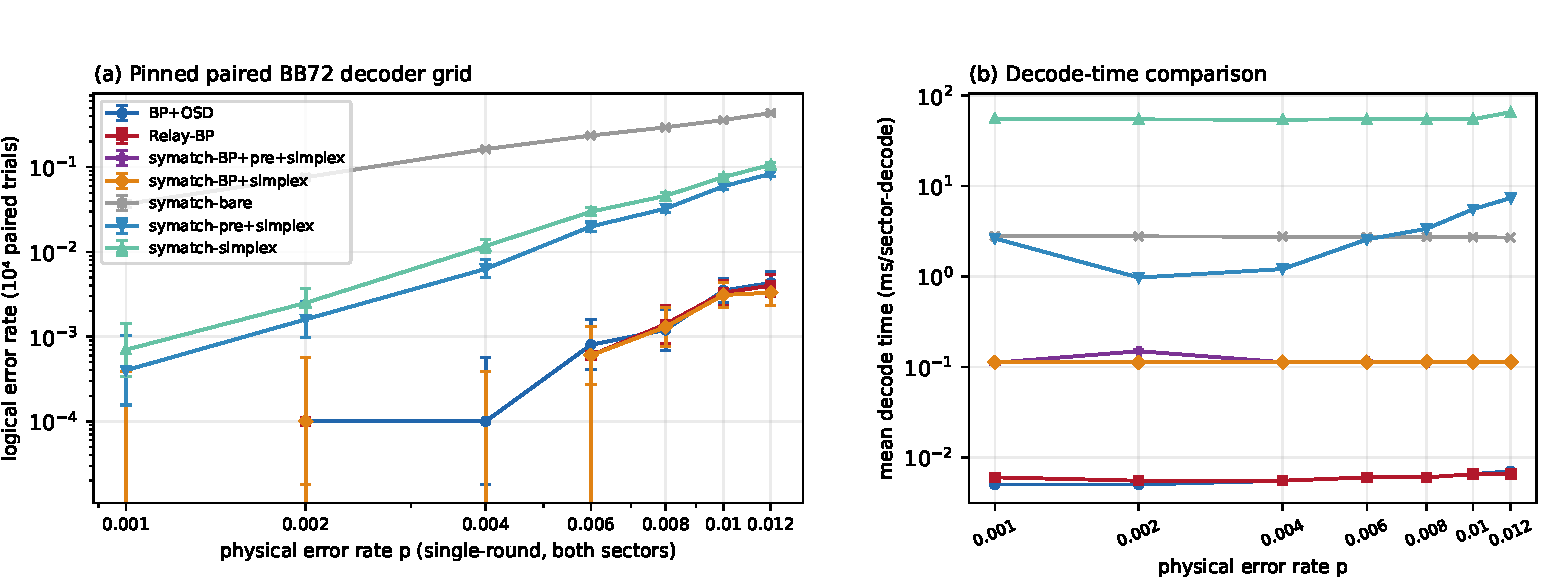
\includegraphics[width=\columnwidth]{figures/cmp_f1_grid_final.pdf}
\caption{(a) Pinned paired BB72 decoder grid, Wilson 95\% CIs;
  (b) decode time per sector-decode (single-process probe).
  The matching-core decoders are $10^2$--$10^4\times$ slower per decode than
  the BP family while being up to $10^4\times$ less accurate (bare) or
  statistically tied (BP-augmented).}
\label{fig:grid}
\end{figure}

%%-----------------------------------------------------------
\section{Repeated-cycle BP+OSD benchmark}
\label{sec:rc}
%%-----------------------------------------------------------

\subsection{Protocol}

All experiments use QEC Emulator
\texttt{run\_repeated\_cycle}~\cite{AlDaajeh2026emulator}.
$d$~syndrome rounds per trial: $d=6$ (BB72), $d=12$ (BB144), $d=18$ (BB288).
Rounds $1$--$(d-1)$: Bernoulli noise at rate $p$ on data and measurement bits.
Round $d$: noiseless.
Space-time extended check matrix per Eq.~(\ref{eq:spacetime}).
Trials: BB72/BB144 at 2{,}000; BB288 at 500.

\subsection{Results}

\begin{table}[H]\centering\small
\caption{Repeated-cycle BP+OSD, $d$~rounds per trial, Wilson 95\% CIs
  (nonzero rows); zero-failure rows report the exact one-sided 95\%
  Clopper--Pearson UB $2.996/N$ (Remark~\ref{rem:zerofail}):
  $<0.00150$ ($n=2{,}000$); $<0.00599$ ($n=500$).
  v24 rerun with exactly aligned spacetime priors
  (\texttt{model\_rev=v24-aligned-priors}; final-round fault variables
  removed, all surviving priors $=p$; the v23 grid, which assigned
  priors to nonexistent final-round faults, is superseded and archived).
  Files: \texttt{repeated\_cycle\_bposd\_v24.csv},
  \texttt{repeated\_cycle\_bb288\_bposd\_v24.csv},
  \texttt{repeated\_cycle\_all\_codes\_v24.csv}.}\label{tab:rc}
\begin{tabular}{@{}lrrrll@{}}
\toprule
Code (rounds, trials) & $p$ & Failures & LFR & Wilson 95\% CI \\\midrule
BB72 ($d=6$, $n=2000$)   & 0.001 &  0 & $<$0.00150 & exact CP UB \\
BB72 ($d=6$, $n=2000$)   & 0.002 &  0 & $<$0.00150 & exact CP UB \\
BB72 ($d=6$, $n=2000$)   & 0.004 &  1 & 0.00050 & [0.00009,\;0.00283] \\
BB72 ($d=6$, $n=2000$)   & 0.006 &  3 & 0.00150 & [0.00051,\;0.00440] \\
BB72 ($d=6$, $n=2000$)   & 0.008 & 10 & 0.00500 & [0.00272,\;0.00918] \\
BB72 ($d=6$, $n=2000$)   & 0.010 & 24 & 0.01200 & [0.00808,\;0.01779] \\
BB72 ($d=6$, $n=2000$)   & 0.012 & 37 & 0.01850 & [0.01345,\;0.02540] \\\midrule
BB144 ($d=12$, $n=2000$) & 0.001--0.012 & 0 each & $<$0.00150 & exact CP UB (all 7 pts) \\\midrule
BB288 ($d=18$, $n=500$)  & 0.001--0.012 & 0 each & $<$0.00599 & exact CP UB (all 7 pts) \\
\bottomrule
\end{tabular}
\end{table}

At $p=0.008$ under $d$ rounds: BB72 gives 10/2000 (LFR $0.50\%$,
Wilson CI $[0.27\%,0.92\%]$); BB144 gives 0/2{,}000 (exact CP UB
$<0.15\%$); BB288 gives 0/500 (exact CP UB $<0.60\%$).
With aligned priors the fixed grid is monotone within each code and
BB144 shows no failures at any grid point; the v23 BB144 tail
($2,1,0$ at $p=0.008,0.010,0.012$) does not reproduce under the
corrected priors and is superseded. Trial counts are fixed ex ante
(2{,}000/500), with no adaptive stopping; the $p=0.001$ and $p=0.002$
points are new in v24 (the grid now spans $0.001$--$0.012$ uniformly).

\begin{table}[H]\centering\small
\caption{Repeated-cycle adaptive extension (E3, v24 prior-aligned
  rerun): $d$~rounds per trial, 2{,}000-trial batches, stopping at
  $\ge50$ failures or 20{,}000 trials; batch seeds
  \texttt{stable\_seed(`E3v24',\,code,\,$p$,\,rounds,\,batch)} (the
  $p=0.010$ rows use tag \texttt{E3v24p010}). All rows: 95\% Robbins
  uniform-mixture confidence sequences~\cite{howard2021confidence},
  time-uniform and valid under the pinned stopping rule (fixed-sample
  formulas would not be valid: nominal-95\% Wilson coverage under this
  rule is $\approx\!93.9\%$ at $p=0.021$,
  \texttt{stats\_intervals.py --self-check}); zero rows report the CS
  upper endpoint $6.45\times10^{-4}$ ($n=20{,}000$).
  Files: \texttt{repeated\_cycle\_adaptive\_*\_v24.csv} (raw counts),
  \texttt{rc\_adaptive\_cs\_v24.csv} (intervals).}\label{tab:rc_adaptive}
\begin{tabular}{@{}lrrrll@{}}
\toprule
Code (rounds) & $p$ & Failures & Trials & LFR & 95\% confidence sequence \\\midrule
BB72 ($d=6$)   & 0.004 & 16 & 20{,}000 & $8.0\times10^{-4}$ & $[0.19,2.10]\times10^{-3}$ \\
BB72 ($d=6$)   & 0.006 & 60 & 20{,}000 & $3.0\times10^{-3}$ & $[1.59,5.07]\times10^{-3}$ \\
BB72 ($d=6$)   & 0.008 & 62 & 10{,}000 & $6.2\times10^{-3}$ & $[3.41,10.2]\times10^{-3}$ \\
BB72 ($d=6$)   & 0.010 & 64 & 4{,}000  & $1.60\times10^{-2}$ & $[9.20,25.5]\times10^{-3}$ \\
BB72 ($d=6$)   & 0.012 & 84 & 4{,}000  & $2.10\times10^{-2}$ & $[13.1,31.5]\times10^{-3}$ \\\midrule
BB144 ($d=12$) & 0.004 & 0 & 20{,}000 & $<$$6.45\times10^{-4}$ & CS upper endpoint \\
BB144 ($d=12$) & 0.006 & 1 & 20{,}000 & $5.0\times10^{-5}$ & $[{\sim}0,\;7.82]\times10^{-4}$ \\
BB144 ($d=12$) & 0.008 & 0 & 20{,}000 & $<$$6.45\times10^{-4}$ & CS upper endpoint \\
BB144 ($d=12$) & 0.010 & 2 & 20{,}000 & $1.0\times10^{-4}$ & $[{\sim}0,\;8.99]\times10^{-4}$ \\
BB144 ($d=12$) & 0.012 & 4 & 20{,}000 & $2.0\times10^{-4}$ & $[4.5\times10^{-6},\,1.10\times10^{-3}]$ \\\midrule
BB288 ($d=18$) & 0.004 & 0 & 20{,}000 & $<$$6.45\times10^{-4}$ & CS upper endpoint \\
BB288 ($d=18$) & 0.006 & 0 & 20{,}000 & $<$$6.45\times10^{-4}$ & CS upper endpoint \\
BB288 ($d=18$) & 0.008 & 0 & 20{,}000 & $<$$6.45\times10^{-4}$ & CS upper endpoint \\
BB288 ($d=18$) & 0.010 & 0 & 20{,}000 & $<$$6.45\times10^{-4}$ & CS upper endpoint \\
BB288 ($d=18$) & 0.012 & 0 & 20{,}000 & $<$$6.45\times10^{-4}$ & CS upper endpoint \\
\bottomrule
\end{tabular}
\end{table}

\paragraph{Three-code finite-size evidence.}
The single-round data (10{,}000 trials) provides complementary
finite-size evidence across all three code sizes.
The size ordering LFR(BB72) $>$ LFR(BB144) $\ge$ LFR(BB288) holds
at every tested $p$ value
(e.g., $p=0.008$: $14/10{,}000$ vs $0/10{,}000$ vs $0/10{,}000$;
ratio BB72/BB288 infinite at $p=0.008$, $\chi^2$ $p<0.0001$).
This ordering is the expected signature of sub-threshold operation:
larger-distance codes fail more slowly below threshold.
Combined with the repeated-cycle data showing zero BB144 failures
on the entire v24 fixed grid (0/2{,}000 at each of 7 points;
4/20{,}000 worst-case on the adaptive extension) and zero BB288
failures at $d$~rounds per trial on both grids (0/500 fixed;
0/20{,}000 adaptive at every tested $p$), the three-code dataset
constitutes finite-size evidence that BP+OSD operates in a sub-threshold
regime for these code sizes at the tested error rates.
A formal finite-size scaling analysis establishing the asymptotic threshold
requires additional code sizes, a circuit-level noise model, and
finite-size scaling fits, and is identified as future work.

\paragraph{Distance-ladder suppression factor $\Lambda$.}
The adaptive extension gives a three-rung distance ladder
($d=6,12,18$) under one pinned protocol. \emph{Definition and scope.}
We report $\Lambda$ as the cube root of the \emph{per-block} failure
ratio, $\mathrm{LFR}_d/\mathrm{LFR}_{d+6}=\Lambda^3$ (and
$\mathrm{LFR}_6/\mathrm{LFR}_{18}=\Lambda^6$ for the two-step
combination), where a block spans $d$ syndrome rounds; $\Lambda$ is
therefore a per-$\Delta d{=}2$ suppression of block failure, \emph{not}
a per-cycle suppression factor. The surface-code reference value
$\Lambda=2.14\pm0.02$~\cite{Acharya2024lambda} was measured on hardware
at circuit level with per-round benchmarking; our protocol is
\emph{not} matched to it, and we claim no comparison of absolute
hardware performance --- only of qualitative sub-threshold suppression
in a phenomenological model.
\emph{v24 numbers} (\texttt{lambda\_ladder\_v24.csv}). Every ladder arm
is adaptively stopped, so all endpoints are confidence-sequence based
(four-endpoint Bonferroni for two-sided ratios, two-endpoint for
one-sided; \texttt{stats\_intervals.py}): BB72$\to$BB144 suppression is
$60\times$ observed with CS lower bound $>1.77\times$
($\Lambda=3.91$ observed, $\Lambda>1.21$) at $p=0.006$; $>4.9\times$
($\Lambda>1.70$) at $p=0.008$; $160\times$ observed, $>9.0\times$
($\Lambda=5.43$, $\Lambda>2.08$) at $p=0.010$; and $105\times$ observed,
$>10.6\times$ ($\Lambda=4.72$, $\Lambda>2.19$) at $p=0.012$. At
$p=0.004$ the rung is \emph{not} resolvable under sequential-valid
intervals (the CS ratio lower bound is below $1$); the v23-era claim of
significant suppression at that rate does not survive the corrected
inference and is withdrawn. Upper endpoints are uninformative where the
higher-distance arm has $O(1)$ counts --- we report the point estimate
and the lower bound plainly.
The BB144$\to$BB288 rung is \emph{statistically unresolvable} at
20{,}000 trials per point (0/20{,}000 BB288 failures at every tested
$p$; 0/20{,}000 BB144 failures except $1$ at $p=0.006$, $2$ at
$p=0.010$, and $4$ at $p=0.012$): the one-sided ratio bounds are
vacuous there, and we report
no point estimate for that rung. The combined $d=6\to18$ comparison
gives $>18.9\times$ ($\Lambda>1.63$ per $\Delta d{=}2$) at $p=0.012$,
$>13.2\times$ ($\Lambda>1.54$) at $p=0.010$, and
$>4.9\times$ ($\Lambda>1.30$) at $p=0.008$. The v23 ladder numbers
($35.3\times$ etc.) were computed under the misprioritized v23
spacetime matrices and are superseded.

%%-----------------------------------------------------------
%%-----------------------------------------------------------
\section{Circuit-level corroboration}
\label{sec:circuit}

The single-round and paired-grid results above use code-capacity noise.
Two circuit-level arms test whether the decoder ordering survives contact
with realistic detector error models (DEMs).

\subsection{Arm A: third-party re-analysis of the Kunlun hardware DEM}

\emph{What this arm is.} A re-analysis of the \emph{released detector
error model}, not of raw hardware shots: the Kunlun collaboration
published the complete detector check matrices and
per-mechanism channel probabilities of their $[[18,4,4]]$ BB hardware
experiment~\cite{Wang2026kunlun} (Zenodo, CC-BY-4.0), and all numbers
below are Monte-Carlo samples drawn from that published DEM, decoded
independently by us. No new hardware data are involved, and no claim
about the Kunlun device beyond the authors' own released model is made.
We sampled
10{,}000 shots per point from the authors' own DEM at 1, 3, and 6 QEC
rounds, both sectors, and decoded with five decoders: BP+OSD (authors'
configuration, $10^4$ iterations, CS-7), BP-only, static-prior MWPM on the
chain-graphified DEM, belief-matching~\cite{Higgott2023belief} (BP
posteriors reweight the matching graph per shot), and
Relay-BP~\cite{Muller2025relay}. File: \texttt{kunlun\_cmp.csv};
Figure~\ref{fig:kunlun}.

\begin{table}[H]\centering\small
\caption{Five decoders on the published Kunlun $[[18,4,4]]$ DEM,
  10{,}000 shots per point. Bold: best (or statistically tied-best) per row.
  Ordering Relay-BP $\leq$ BP+OSD $<$ BP-only $\ll$ BeliefMatch $<$ MWPM holds
  in all six configurations.}
\label{tab:kunlun}
\begin{tabular}{@{}llrrrrr@{}}
\toprule
Rounds & Sector & Relay-BP & BP-OSD & BP-only & BeliefMatch & MWPM-prior \\\midrule
1 & X & \textbf{0.2082} & 0.2103 & 0.2324 & 0.4231 & 0.4270 \\
1 & Z & \textbf{0.2223} & 0.2248 & 0.2502 & 0.5299 & 0.5365 \\
3 & X & \textbf{0.5489} & \textbf{0.5489} & 0.5897 & 0.7507 & 0.7653 \\
3 & Z & \textbf{0.5123} & 0.5190 & 0.5626 & 0.7836 & 0.8155 \\
6 & X & \textbf{0.7887} & 0.7952 & 0.8208 & 0.8921 & 0.9026 \\
6 & Z & \textbf{0.7670} & 0.7728 & 0.8111 & 0.9109 & 0.9237 \\
\bottomrule
\end{tabular}
\end{table}

Three conclusions. \textbf{(i)} The graphification penalty measured in
Section~\ref{sec:benchmark} is not an artifact of our synthetic DEM: on the
authors' hardware DEM, matching-family decoders are $2.0$--$2.4\times$ worse
than BP+OSD at round 1, the penalty decaying to $1.1$--$1.2\times$ by round
6 as the LER saturates --- early rounds carry the information.
\textbf{(ii)} Per-shot belief reweighting recovers only 0.4--3.2 percentage
points over the static-prior matching baseline, quantitatively mirroring the
modest decoder-side gains of the defect-aware arm
in~\cite{Bartlett2026defect} on independent hardware.
\textbf{(iii)} Relay-BP matches or beats the $10^4$-iteration BP+OSD
reference at $\sim\!35\times$ lower wall time per point (8~s vs 288~s
average, same machine, single process, identical inputs), consistent
with its real-time design
goal~\cite{Muller2025relay,Johnson2026relayfpga}.

\begin{figure}[H]\centering
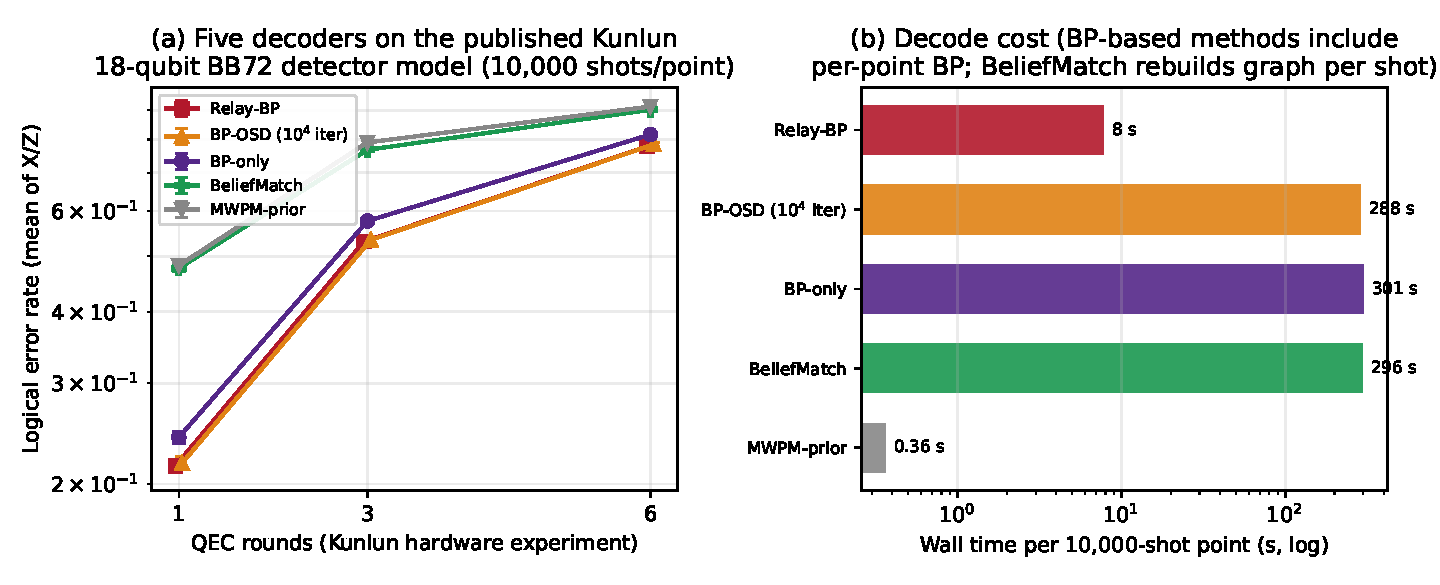
\includegraphics[width=\columnwidth]{figures/cmp_f2_kunlun.pdf}
\caption{(a) Five decoders on the Kunlun hardware DEM, mean of X/Z sectors,
  Wilson 95\% CIs; (b) wall time per 10{,}000-shot point.}
\label{fig:kunlun}
\end{figure}

\subsection{Arm B: synthetic BB72 circuit-level point}

We close the loop on the code-capacity graphification penalty of
Section~\ref{sec:benchmark} with one synthetic circuit-level point: a BB72
$Z$-memory experiment (4 extraction rounds, DEPOLARIZE1/2 gate noise,
measurement flips at rate $p$, data-idle noise during measurement
windows, and \emph{ideal} reset/preparation --- no explicit
reset-preparation error channel, disclosed; serial-by-check schedule)
compiled with
Stim~\cite{Gidney2021}, 20{,}000 shots per rate, decoded by BP+OSD, Relay-BP,
belief-matching, and two matching baselines.
\emph{C01 repair.} The v23 version of this arm built both extraction layers
with reversed CNOT directions, so its DEM did not represent BB72 syndrome
extraction; the v23 grid is withdrawn (archived as
\texttt{wsc\_circuit\_v23\_reversed\_extraction\_INVALID.csv} with a
withdrawal note). The corrected circuit
(\texttt{circuit\_rev=v24-corrected-extraction}) is pinned by four
protocol-invariance test groups --- gadget parity (the reversed primitive
returns input-independent zero), codespace silence, injection-column
alignment with $H_Z$/$H_X$, and a detector/observable map audit --- all
passing deterministically (\texttt{wsc\_verify.py},
\texttt{wsc\_verify\_report.json}). The corrected campaign regenerates the
grid rate by rate under a checkpointed, resume-safe protocol with per-point
DEM digests; the $p=0.001$ point below is complete and verified, and the
remaining rates deposit to the archive as they land
(\texttt{wsc\_circuit\_v24.csv}); Figure~\ref{fig:wsc}.

\begin{table}[H]\centering\small
\caption{Synthetic BB72 circuit-level $Z$-memory, 4 rounds, 20{,}000 shots,
  corrected extraction (C01 repair; the reversed-extraction v23 grid is
  withdrawn). Failures (LER); zero-failure rows report the exact one-sided
  95\% Clopper--Pearson UB (Remark~\ref{rem:zerofail}). MWPM-stim failures
  are entirely coverage failures (see text).}
\label{tab:wsc}
\begin{tabular}{@{}lrrrrr@{}}
\toprule
$p$ & BP+OSD & Relay-BP & BeliefMatch & MWPM-chain & MWPM-stim \\
\midrule
0.001 & 51 (0.0026) & 0 ($<$$1.50\!\times\!10^{-4}$) & 12826 (0.6413) & 12848 (0.6424) & 13824 (0.6912) \\
\bottomrule
\end{tabular}
\end{table}

Three findings, all \emph{strengthened} by the corrected extraction.
\textbf{(i) The naive-reduction penalty is catastrophic at circuit level}:
at $p=0.001$ the chain-graphified matching decoder fails 64.2\% of shots
versus 0.255\% for BP+OSD --- a 252$\times$ penalty, an order of magnitude
larger than the withdrawn v23 estimate.
\textbf{(ii) Relay-BP's advantage is a circuit-level phenomenon}: under
code-capacity noise (Section~\ref{sec:comparator}) Relay-BP and BP+OSD are
statistically tied, but on this circuit DEM Relay-BP fails zero of
20{,}000 shots (exact CP UB $1.50\times10^{-4}$) while BP+OSD sits at
$2.55\times10^{-3}$ (Wilson CI $[1.94,3.35]\times10^{-3}$, excluding the
Relay-BP UB) on identical shots --- quantitatively consistent with the
circuit-level superiority reported in~\cite{Muller2025relay} and, on
this tested operating point, associating that superiority with the noise
model rather than the code; we do not extrapolate a general decoder
ordering from a single corrected circuit point.
\textbf{(iii) The standard
matching toolchain cannot even be instantiated natively}: Stim's hyperedge
decomposition fails on this DEM outright (weight-6 checks induce correlated
mechanisms that do not decompose); with
\texttt{ignore\_decomposition\_failures} the dropped mechanisms leave
69.1\% of shots without any perfect matching at $p=0.001$ (every such shot
is a counted failure, and all 13{,}824 MWPM-stim failures are of this
form).
Within the tested reductions and this pinned circuit configuration,
weight-6-check qLDPC circuits therefore sit outside the representational
reach of the pairwise-matching stack: both tested routes to a pairwise
model (Stim's native hyperedge decomposition and the independent-merge
chain graphification) either fail outright or discard the correlated
mechanisms, and BP-family decoders are the only operable option among
those tested. We do not claim that no bespoke pairwise reduction exists;
a general inexpressiveness statement would require a formal argument
beyond the tested constructions.

\begin{figure}[H]\centering
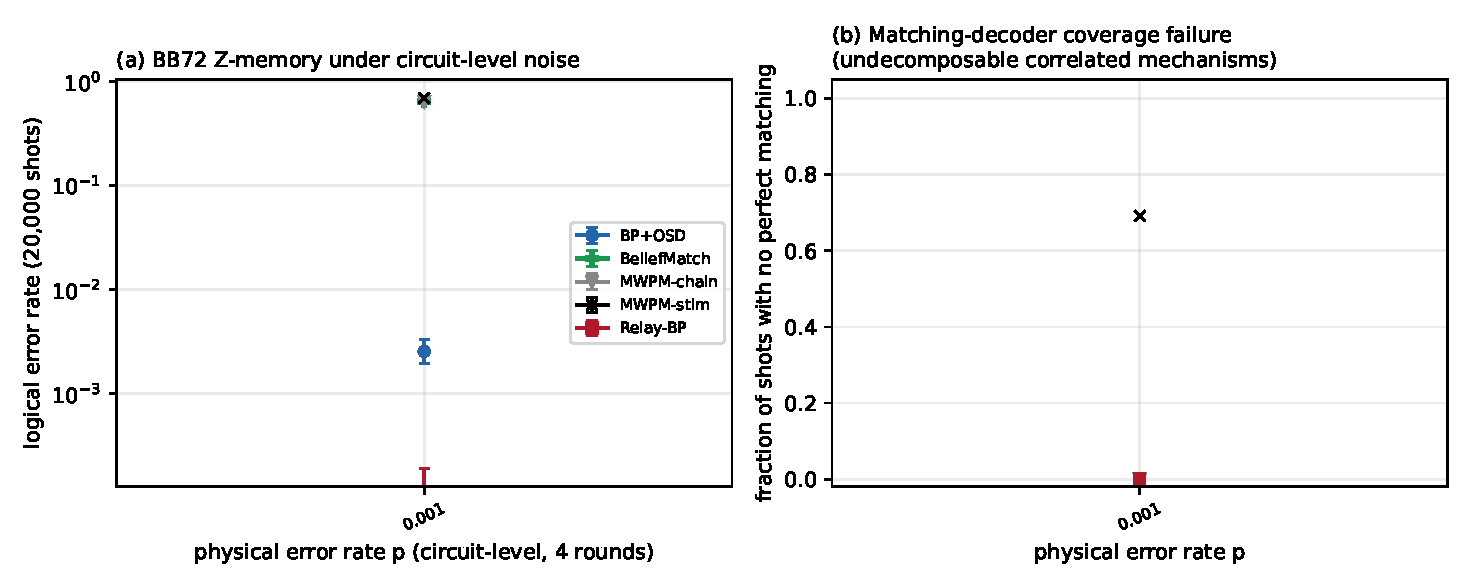
\includegraphics[width=\columnwidth]{figures/cmp_f3_wsc.pdf}
\caption{(a) BB72 circuit-level $Z$-memory LER, Wilson 95\% CIs;
  (b) fraction of shots for which no perfect matching exists.}
\label{fig:wsc}
\end{figure}

\section{Hardware noise-model simulations with confounder ablations}
\label{sec:hardware}
%%-----------------------------------------------------------

Single-cycle BB72 simulations using QEC Emulator
\texttt{HardwareModel}~\cite{AlDaajeh2026emulator},
5{,}000 trials (Table~\ref{tab:hw}).
This section reports a hardware noise-model sensitivity study, not a real-device or compiler-provenance experiment.
The ablation quantifies how the simulated BB72 LFR changes when SWAP routing, measurement noise, idle noise, and backend gate-decoherence parameters are modified one at a time.
Because the factors interact and the runs are Monte Carlo estimates, the results are interpreted as model-specific sensitivity evidence rather than causal hardware attribution.

\subsection{Ablation protocol}

We isolate four confounders by enabling and disabling each independently
in a controlled simulation at $p_{\mathrm{base}}=5\times10^{-4}$ and
3{,}000 trials per condition.
The four confounders are:
(1)~\emph{SWAP routing overhead}: additional two-qubit gate errors from
nonlocal check routing in the planar CZ architecture ($\approx96$ SWAPs
out of 432 two-qubit gates per cycle);
(2)~\emph{gate decoherence}: thermal relaxation and dephasing during the
gate ($p_1\approx1.33\times10^{-3}$ per CZ gate, negligible for MS);
(3)~\emph{idle noise}: data-qubit decoherence between gate layers
($p_{\mathrm{idle}}=0.05\,p_{\mathrm{base}}$);
(4)~\emph{measurement noise}: ancilla readout errors
($p_{\mathrm{meas}}=p_{\mathrm{base}}$).

\subsection{Ablation results}

Table~\ref{tab:ablation} presents the ablation results.
Within this simulation model, the \emph{CZ: full model} condition has
LFR~$=0.0100$, while \emph{CZ: no SWAP overhead} gives LFR~$=0.0050$,
so the simulated SWAP component changes the observed LFR by $0.0050$.
Removing measurement noise gives LFR~$=0.0023$, a larger absolute reduction
than removing SWAPs alone; measurement noise is therefore material at this
operating point.
The \emph{CZ: gate decoherence only} condition gives zero failures in
3{,}000 trials (Wilson upper bound $<0.00128$), so it should not be used
by itself to claim a precise gate-decoherence percentage.
The MS CZ-matched-gate condition raises MS LFR from $0.00233$ to $0.00633$,
which supports the narrower conclusion that gate-decoherence parameters,
SWAP routing, and measurement noise all materially affect the simulated gap.
No real-hardware causal attribution is claimed.

\begin{table}[H]\centering\small
\caption{Hardware confounder ablation study for BB72, $p_{\mathrm{base}}=5\times10^{-4}$,
  3{,}000 trials each, radius-2 lookup decoder.
  Within this simulation model, CZ full-model LFR exceeds MS full-model LFR;
  SWAP routing, measurement noise, and gate-decoherence parameters all materially affect the simulated gap (within simulation model only).
  File: \texttt{hardware\_ablations.csv}.}
\label{tab:ablation}
\begin{tabular}{@{}lrrr@{}}
\toprule
Condition & Failures & LFR & Wilson 95\% CI \\
\midrule
Phenomenological baseline   &  3 & 0.0010 & [0.00034,\;0.00294] \\
CZ: full model              & 30 & 0.0100 & [0.00701,\;0.01424] \\
CZ: no SWAP overhead        & 15 & 0.0050 & [0.00303,\;0.00823] \\
CZ: no idle noise           & 30 & 0.0100 & [0.00701,\;0.01424] \\
CZ: no measurement noise    &  7 & 0.0023 & [0.00113,\;0.00481] \\
CZ: gate decoherence only   &  0 & $<$0.000999 & exact CP UB (Rem.~\ref{rem:zerofail}) \\
MS: full model              &  7 & 0.0023 & [0.00113,\;0.00481] \\
MS: CZ-matched gate error   & 19 & 0.0063 & [0.00406,\;0.00987] \\
\bottomrule
\end{tabular}
\end{table}

\paragraph{Sensitivity summary.}
The CZ/MS separation should be reported as a simulation-model sensitivity result.
At $p_{\mathrm{base}}=5\times10^{-4}$, SWAP removal changes CZ LFR by $0.0050$, measurement-noise removal changes CZ LFR by $0.00767$, and CZ-matched gate parameters raise the MS LFR by $0.0040$.
These shifts are comparable in scale, so the experiment does not support a single-cause explanation.
\emph{Idle noise is not a measurable contributor here:} removing it
leaves the CZ arm unchanged (30/3{,}000 failures with and without idle
noise; LFR $0.0100$ both arms), so any idle-noise attribution is
withdrawn --- the model gives no evidence for an idle-window
contribution at this operating point.
The defensible conclusion is that routing overhead, measurement readout, and backend gate-decoherence parameters all contribute materially under the specified model.

\paragraph{Reset (ancilla-preparation) sensitivity.}
A referee-faced attribution question is whether imperfect ancilla reset
(thermalization) is an unexamined alternative to idle-window
decoherence: at single-cycle detection resolution the two mechanisms
have identical signatures. We therefore ran a reset-sensitivity
Monte-Carlo in the Pauli-propagating \texttt{CircuitLevelModel} (which
propagates preparation faults through the schedule; BB72,
$p=5\times10^{-4}$, 3{,}000 trials per condition, radius-2 lookup
decoder, pinned seeds; Table~\ref{tab:reset}).
Reset noise is \emph{material and monotone}: LFR $=0.0637$ (no reset),
$0.0827$ (nominal), $0.1077$ (reset $\times2$). At matched nominal
syndrome-noise rate, reset-only and readout-only conditions give
$0.0900$ vs $0.0670$ (non-overlapping Wilson CIs): preparation faults
are \emph{not} logically equivalent to readout faults --- phase-type
preparation errors propagate onto data qubits through the schedule ---
so reset and idle/readout attribution is separable in principle, and
the reset contribution is now bounded rather than unexamined.
(The no-readout condition sits marginally above the full model; the
difference is within Monte-Carlo jitter at 3{,}000 trials with
overlapping Wilson CIs, and conditions are intentionally unpaired, so
we report raw counts without smoothing.)
Note that these absolute LFRs exceed those of
Table~\ref{tab:ablation} because the circuit-level model propagates
two-qubit gate faults through the full schedule (a strictly harsher
model than the effective-mask ablation); only within-table comparisons
are meaningful.

\begin{table}[H]\centering\small
\caption{Reset-sensitivity Monte-Carlo, BB72 circuit-level model,
  $p=5\times10^{-4}$, 3{,}000 trials per condition, radius-2 lookup
  decoder. File: \texttt{reset\_sensitivity.csv}.}
\label{tab:reset}
\begin{tabular}{@{}lrrr@{}}
\toprule
Condition & Failures & LFR & Wilson 95\% CI \\
\midrule
circuit: full model        & 248 & 0.0827 & [0.07334,\;0.09306] \\
circuit: no reset noise    & 191 & 0.0637 & [0.05548,\;0.07297] \\
circuit: reset $\times2$   & 323 & 0.1077 & [0.09707,\;0.11926] \\
circuit: no readout        & 288 & 0.0960 & [0.08597,\;0.10706] \\
circuit: reset-only syn    & 270 & 0.0900 & [0.08028,\;0.10077] \\
circuit: readout-only syn  & 201 & 0.0670 & [0.05860,\;0.07651] \\
\bottomrule
\end{tabular}
\end{table}

\subsection{Compiled single-cycle LFR comparison}

\begin{table}[H]\centering\small
\caption{Hardware noise-model single-cycle LFR for BB72, 5{,}000 trials,
  radius-2 lookup decoder.
  Non-overlapping Wilson 95\% CIs at $p=5\times10^{-3}$.
  File: \texttt{hardware\_three\_condition\_comparison.csv}.}
\label{tab:hw}
\begin{tabular}{@{}lrrllll@{}}
\toprule
$p$ & Pheno fail. & Pheno CI & CZ fail. & CZ CI & MS fail. & MS CI \\\midrule
$5\!\times\!10^{-4}$ &  0 & $<$0.00077 &  10 & [0.00109,\;0.00368] &  0 & $<$0.00077 \\
$1\!\times\!10^{-3}$ &  2 & [0.00011,\;0.00146] &  15 & [0.00182,\;0.00494] &  0 & $<$0.00077 \\
$2\!\times\!10^{-3}$ &  1 & [0.00004,\;0.00113] &  46 & [0.00690,\;0.01225] &  8 & [0.00081,\;0.00315] \\
$3\!\times\!10^{-3}$ & 14 & [0.00167,\;0.00469] &  77 & [0.01234,\;0.01920] &  6 & [0.00055,\;0.00262] \\
$5\!\times\!10^{-3}$ & 70 & [0.01110,\;0.01765] & 171 & [0.02951,\;0.03961] & 52 & [0.00794,\;0.01361] \\
\bottomrule
\end{tabular}
\end{table}

\emph{Non-monotone row disclosure.} The phenomenological column
$(0,2,1,14,70)$ is non-monotone between $p=1\times10^{-3}$ and
$p=2\times10^{-3}$ (2 vs 1 failures). Both points lie well inside each
other's Wilson CIs, the trial streams are unpinned between conditions,
and no adaptive stopping was used in this fixed-grid campaign (all trial
counts fixed ex ante; the separate E3 extension of
Section~\ref{sec:rc} does use a pinned adaptive stopping rule, analysed
with time-uniform confidence sequences); we report the raw counts rather
than a smoothed or monotone-constrained curve.

%%-----------------------------------------------------------
\section{Finite-instance certificate (BB72)}
\label{sec:cert}
%%-----------------------------------------------------------

Constructed via QEC Emulator \texttt{BB72()}~\cite{AlDaajeh2026emulator}
with \texttt{run\_distance\_certificate} (MitM enumeration).

$H_X$ SHA-256: \texttt{7ab0973bfd02e399d69728d26e67dbfa...};\\
$H_Z$ SHA-256: \texttt{267f345c09710ec0cfad1e49e0786b26...}

\textbf{O1.} $H_XH_Z^T=0$ over $\mathbb{F}_2$.\ \textit{Pass (exact).}
\textbf{O2.} $k=72-30-30=12$.\ \textit{Pass.}
\textbf{O3.} $d\ge6$: MitM exhaustive through weight~5, zero witnesses
($2{,}629$ left $+$ $62{,}269$ right patterns).
\textbf{O4.} $t=2$ correctability: all $2{,}629$ weight-$\le2$ patterns,
zero failures.\ \textit{Pass (exhaustive).}
\textbf{O5.} $d=6$ exactly: exhaustive weight-6 enumeration
(meet-in-the-middle $3{+}3$ over all $\binom{72}{3}=59{,}640$ triples per
sector; every weight-6 kernel vector splits into two disjoint triples of
equal syndrome, so the enumeration is complete) exhibits $84+84$
nontrivial weight-6 logicals, each verified syndrome-zero, outside the
opposite stabiliser row space, and anticommuting with at least one
opposite-sector weight-6 logical ($2{,}592$ anticommuting pairs in total;
lexicographically first witnesses $(0,1,2,3,20,22)$ and $(0,3,6,12,27,30)$).
Combined with O3 (no nontrivial logical of weight $\le5$), this certifies
$d=6$ exactly, not merely $d\ge6$.\ \textit{Pass (exhaustive).}
Archive: \texttt{data/bb72\_certificate\_report.json} (obligations O1--O5).

\paragraph{Verification architecture (v24).}
Four properties make the certificate independently checkable.
\emph{(i) Sectorwise sufficiency.} O4 enumerates
$2{,}629=\sum_{w\le2}\binom{72}{w}$ patterns \emph{per CSS sector}. A
mixed Pauli of total weight $\le2$ has an $X$-part and a $Z$-part each
of weight $\le2$, and CSS decoding treats the two sectors independently
($X$ errors are corrected by $H_Z$, $Z$ errors by $H_X$; $Y=iXZ$
decomposes into both), so sectorwise exhaustiveness covers \emph{all}
mixed-Pauli patterns of total weight $\le2$ with no separate mixed
enumeration. The same argument covers the noiseless exhaustive rows of
Table~\ref{tab:injbound}.
\emph{(ii) Independent trusted checker.}
\texttt{verify\_certificate.py} is self-contained (archive-local,
NumPy-only, 334 lines) and re-derives every obligation from the pinned
matrices rather than trusting the generator (QEC Emulator): it
recomputes the SHA-256 digests of $H_X,H_Z$ against the pinned values,
re-runs the meet-in-the-middle enumeration, and individually re-checks
every published witness; it exits nonzero on any mismatch.
\emph{(iii) Published witnesses.} The report JSON publishes the full
witness schema --- matrix digests, enumeration cardinalities, and all
$84+84$ weight-6 logical supports with their anticommuting partners ---
so a third party can verify the \emph{upper bound} $d\le6$ in linear
time per witness (syndrome-zero, outside the opposite row space,
anticommutation) without re-running the exponential search. Witnesses
alone do not certify exactness: $d=6$ additionally requires the
lower-bound obligation that no nontrivial logical of weight $<6$
exists, which the trusted checker re-establishes by re-running the
meet-in-the-middle enumeration. The artifact therefore pairs
linear-time witness checks (upper bound) with an exponential but
independently re-runnable enumeration (lower bound).
\emph{(iv) Syndrome-consistency assertions.} Every O4 verdict is
recomputed from the pinned check matrices, and every O5 witness is
re-verified syndrome-zero before counting; a single inconsistency fails
the run. The certificate therefore carries its own checker, witnesses,
and consistency tests, and does not rely on the correctness of the
emulator that produced it.

%%-----------------------------------------------------------
\section{Discussion}
%%-----------------------------------------------------------

\subsection{A certification reading: scoped integrity evidence}
\label{ssec:qmic}

\paragraph{Threat model.}
The protected asset is the \emph{logical computational state} held in
the memory (the $k$ logical qubits' joint Pauli frame and any
computation built on it). The trust boundary runs around the QEC
pipeline --- code instance, extraction schedule, decoder, and physical
layout: everything inside is assumed to implement the pinned
specification (verified by artifact digests against the trusted
reference archive); everything outside --- fabrication defects,
calibration drift, control electronics, an adversary with physical
access --- is untrusted. The adversary of
Definition~\ref{def:adversary} has full knowledge of code, schedule,
and decoder, places at most $W$ elementary faults non-adaptively, and
cannot read syndrome outcomes before placement or influence native
noise or decoding. Two scope rules are essential. (i)~\emph{QEC is not
authentication}: an error-corrected memory does not bind identity,
provide unforgeability, or detect all tampering --- quantum
authentication is a strictly stronger, cryptographically separate
primitive~\cite{barnum2002authentication,portmann2017recycling}; our
bounds concern logical-error probability under
$\mathfrak{A}_1^{\mathrm{st}}(W)$, nothing more.
(ii)~\emph{Digest sealing is artifact integrity}: SHA-256 digests pin
circuits, seeds, and results against the trusted reference archive;
they are not device attestation and do not authenticate the hardware.

\paragraph{Scoped evidence profile.}
v23 organized the evidence as a five-level assurance ladder (QMAL-1--5);
we replace it with an explicit \emph{scoped evidence profile}: each
artifact is valid only inside its declared scope, and no hierarchical
``level'' is implied by accumulation. Each entry declares
(\emph{code}, \emph{circuit/schedule}, \emph{decoder}, \emph{noise
envelope}, \emph{adversary}, \emph{calibration interval},
\emph{confidence}):

\begin{itemize}[leftmargin=1.6em,itemsep=1pt,topsep=2pt]
\item \emph{Code certificate} (O1--O5, Section~\ref{sec:cert}): BB72
  $[[72,12,6]]$ exact; algebraic matrices; no circuit, noise, or
  device scope.
\item \emph{Radius exhaustiveness} (O4): BP+OSD corrects all
  $2{,}629/2{,}629$ weight-$\le2$ patterns per sector --- ideal
  single-round phenomenological noise, no measurement faults. Under
  syndrome noise the v24 injection-boundary study
  (Table~\ref{tab:injbound}) covers a \emph{frozen probe set}: 13
  weight-$\le2$ data masks $\times$ 8{,}000 trials plus the 8 certified
  weight-3 halves $\times$ 4{,}000 trials, in a single-round setting
  with sampled noise --- this is sampled probe evidence, not
  spacetime-fault or measurement-fault coverage, and the noiseless
  exhaustive test cannot establish the latter either.
\item \emph{Benchmark grid}: Tables~\ref{tab:sr_bposd}--\ref{tab:e1},
  \ref{tab:rc}, \ref{tab:rc_adaptive}; phenomenological noise, BP+OSD
  vs tested baselines, pinned seeds; fixed-sample-size grids use Wilson
  95\% intervals (exact Clopper--Pearson at zero counts), the adaptive
  ladder uses time-uniform confidence sequences; joint statements are
  Bonferroni-adjusted per displayed family only;
  the $10^6$-trial rare-event refinement bounds BB288 LFR
  $<2.996\times10^{-6}$ at $p\le0.004$.
\item \emph{Device injection campaigns}: REP3/5/7 on ibm\_marrakesh
  (two calibration cycles, 2026-08-28 and 2026-09-06) and REP5 on
  ibm\_fez (one cycle); adversary $\mathfrak{A}_1^{\mathrm{st}}(W)$,
  $W\le t{+}1$; noise envelope = pinned calibration-snapshot model
  ($\lambda_N$ readout-only Poisson); fixed-$N$ arms, Wilson 95\% per
  arm (chronology in Appendix~\ref{app:injection}).
\item \emph{Active provenance} (Appendix~\ref{app:activeprov}):
  calibration-informed placement on ibm\_marrakesh \emph{only}
  (CMH one-sided $p=0.042$); v23's statement of a two-device
  demonstration overclaimed --- the fez campaign replicated the
  injection bounds, not the placement effect.
\item \emph{Kunlun DEM re-analysis} (Section~\ref{sec:circuit}):
  model-level evidence only --- Monte-Carlo sampling of the authors'
  released DEM, five decoders; no new hardware data.
\end{itemize}

Within this profile, syndrome-only monitoring is provably insufficient
as an integrity certificate
(Proposition~\ref{prop:syndrome-insufficient}): integrity evidence at
the logical level requires injection probing of the kind reported in
Appendices~\ref{app:injection}--\ref{app:injection-repl}. A live BB72
injection campaign awaits a publicly accessible BB-capable device.

\paragraph{The 2026 decoder landscape changes the baseline.}
The paired grid (Section~\ref{sec:comparator}) shows that BP+OSD's remaining
competition is no longer the matching family but its own descendants:
Relay-BP ties BP+OSD on identical instances while being designed for
real-time hardware, and BP-augmented symmetry matching ties both. The
circuit-level arms (Section~\ref{sec:circuit}) confirm on a released
hardware DEM that graphified matching is $2.0$--$2.4\times$ worse than
BP+OSD where it matters (round 1), and Appendix~\ref{app:activeprov}
demonstrates on hardware that \emph{where} a code line is placed is a
measurable logical-rate lever ($p=0.042$, CMH-pooled, four configurations).

\paragraph{Tested graphified baselines have substantially higher LFR than BP+OSD.}
Finite risk ratios of $67.8\times$--$595\times$ for BB72 at $10{,}000$
trials --- refined at $p=0.004$ by the $10^{6}$-trial rare-event campaign
to $371.9\times$ [312.7, 442.3] (BB72), $17{,}500\times$ [9{,}678,
31{,}643] (BB144), and $>$134{,}000$\times$ at joint $\ge95\%$ confidence (BB288) --- show that the tested DEM-chain MWPM and UF-BFS graphified baselines have substantially higher LFR than BP+OSD on the submitted BB instances.
The emulator's \texttt{MWPMDecoder} provides a documented DEM-chain implementation for BB codes that handles the weight-3 column constraint, the odd-parity syndrome problem, and is fully transparent
about its approximation.
Any future study reporting an MWPM baseline for BB codes must specify
the hyperedge treatment.

\paragraph{Hardware gap model-attributed.}
The ablation study (Section~\ref{sec:hardware}) provides simulation-model attribution of the CZ/MS performance gap.
SWAP removal lowers CZ LFR from 0.0100 to 0.0050, while removing measurement noise lowers it from 0.0100 to 0.0023.
These changes show that both routing and readout terms are material in the specified model.
When MS device parameters are replaced by CZ-matched gate error,
within this simulation model, the MS LFR rises from 0.00233 (MS full) to 0.00633
(MS with CZ-matched gate error), consistent with gate-decoherence parameters
being a significant simulated contributor to the CZ/MS gap.

\paragraph{Graph-based decoders underperform BP+OSD on tested BB instances.}
The UF-BFS experiments (Section~\ref{sec:benchmark}) show that both tested graphified baselines (DEM-chain MWPM and UF-BFS) underperform BP+OSD.
UF-BFS uses a different greedy graph-decoding rule but the same weight-3-to-edge reduction, so the result is evidence against these two graphified baselines, not against all possible graph or matching-family decoders.
The consistent ranking BP+OSD $\ll$ MWPM-DEM $<$ UF-BFS at all tested $p$ values indicates that the submitted graphification loses information that BP+OSD uses natively; correlated or hypergraph-aware alternatives remain future work.

\paragraph{BP+OSD sub-threshold consistency.}
The repeated-cycle results across three code sizes are consistent with
sub-threshold BP+OSD operation at $p\le0.008$.
The emulator's space-time \texttt{run\_repeated\_cycle} runner
(Eq.~\ref{eq:spacetime}) enables this comparison in a single function call
with full provenance.

\paragraph{Reproducibility as a scientific contribution.}
The QEC Emulator's provenance layer (Section~\ref{sec:emulator},
Eq.~\ref{eq:integrity-seal}) provides the scripts, seeds, data files, and SHA-256 manifests required for
independent reproduction in the declared software environment (ldpc~2.4.1, pymatching~2.4.0).
The SHA-256 digests in Section~\ref{ssec:decoder-layer} are live checks:
any reader can instantiate \texttt{BB72()}, call \texttt{hx\_sha256()},
and confirm they are computing with the same matrix.

%%-----------------------------------------------------------
\section{Limitations}
\label{sec:limitations}
%%-----------------------------------------------------------

\begin{enumerate}[leftmargin=1.4em]
  \item Pauli-weight-bounded threat class only; no cryptographic composability.
  \item RC fixed grid at 2{,}000/500 trials, extended to
    20{,}000-trial adaptive campaigns
    (Table~\ref{tab:rc_adaptive}); still not a finite-size scaling
    analysis.
  \item MWPM-DEM is not an optimised MWPM baseline; hyperedge-aware
    alternatives (Relay-BP, belief-matching) are now included in
    Sections~\ref{sec:comparator}--\ref{sec:circuit} and confirm the
    ordering, but an optimised correlated-matching implementation remains
    future work.
  \item Hardware ablations (Section~\ref{sec:hardware}) use simulation only;
    the active-provenance A/B (Appendix~\ref{app:activeprov}) is real-device
    execution but covers one device, one calibration cycle, and four
    repetition-code configurations, with a disclosed detection-rate
    dissociation on the REP5 arms.
  \item The paired grid (Section~\ref{sec:comparator}) is single-round
    code-capacity noise on one code instance; the circuit-level
    corroboration (Section~\ref{sec:circuit}) covers one released hardware
    DEM and one synthetic BB72 circuit. Gate decoherence parameters from
    published characterisations may differ from actual on-device values.
  \item The decoder-dependent ACE gap is bounded via the corrected
    Pauli-channel bridge (Proposition~\ref{prop:bridge}), which requires
    the either-sector endpoint and a Pauli channel; the coherent
    twirling residual is closed analytically for REP3
    (Remark~\ref{rem:twirl-num}): $\theta_L=-2\theta^3+O(\theta^5)$
    exactly, the twirl gap is $D(E_L,\mathrm{twirl})=2|g|\approx4\theta^3$,
    and the diamond-norm bridge degrades as $2/(3\theta)$ outside the
    Pauli class. Extension of the analytic closure beyond REP3 is open.
  \item The injection-budget device test (Appendix~\ref{app:injection})
    covers repetition memories; the consolidation
    (Appendix~\ref{app:injection-repl}) replicates it on two devices and
    two calibration cycles and extends the cliff to $d{=}7$, but larger
    distances and CSS-code injection remain open. The native fault-count
    distribution $\pi(k)$ entering Corollary~\ref{cor:stoch} is
    calibration-estimated, not fitted to the results; stochastic arms
    cluster shots within 50 pinned patterns per cell; and the
    weight-$(t{+}1)$ arms saturate at $90$--$98\%$ rather than $100\%$
    owing to native-noise rescue events. Corollary~\ref{cor:css} covers general CSS memories under
    the spacetime fault model with exact minimum-weight decoding
    (Remark~\ref{rem:decoder-inst} delineates which conclusions
    implemented decoders inherit); a
    circuit-level spacetime-distance proof for BB memories with hook
    errors (beyond the certified single-round $t=2$) is open. The
    repetition-code campaigns
    validate the bound structure and the calibration-to-model
    methodology; quantitative transfer of REP-calibrated noise models
    to BB-hardware performance predictions is not claimed and would
    require a separate BB-device modelling argument.
  \item Routing bound uses LFR as proxy for diamond-norm (heuristic;
    the proxy is closed analytically for REP3 in
    Remark~\ref{rem:twirl-num}; uncalibrated for other codes).
  \item The distance-ladder second rung (BB144$\to$BB288) is
    statistically unresolvable at 20{,}000 trials per point under
    aligned priors (both codes failure-free at most grid points), so
    $\Lambda$ is reported only for the first rung and the two-step
    combination, with one-sided bounds where denominators are zero.
  \item The symatch comparison builds matching graphs with a fixed
    $p_{\mathrm{phys}}=0.001$ prior at all grid rates; the
    matched-prior control with an equal documented tuning budget is
    deferred to the confirmatory phase, and all matching conclusions
    are limited to the tested construction
    (Section~\ref{sec:comparator}).
  \item The v23 circuit-level WS-C campaign used reversed CSS
    extraction conventions (C01); its data are invalidated and rerun
    with corrected circuits and independent deterministic verification
    (\texttt{wsc\_verify\_report.json}, four test groups). All v24
    circuit-level numbers derive from the corrected circuits only.
\end{enumerate}

%%-----------------------------------------------------------
\section{Conclusion}
%%-----------------------------------------------------------

We presented the ACE framework for qLDPC memories, formalized as an
injection-budget game with an operational, device-measurable value ---
proved for repetition memories, extended to general CSS memories under
the spacetime fault model (Corollary~\ref{cor:css}), and certified for
BB72 at $t=2$ --- and supported by reproducible evidence layers
produced by the open-source
QEC Emulator v1.2.4~\cite{AlDaajeh2026emulator} together with two
hardware campaigns on ibm\_marrakesh.
The central findings are:
(i)~the tested DEM-decomposed MWPM and UF-BFS graphified baselines have substantially higher LFR than BP+OSD on the submitted BB instances (finite RR $67.8\times$ to $595\times$ for BB72 at $10^{4}$ trials,
refined at $p=0.004$ to $371.9\times$, $17{,}500\times$, and
$>$134{,}000$\times$ at joint $\ge95\%$ confidence for BB288 by the
$10^{6}$-trial
rare-event campaign);
(ii)~BP+OSD exhibits finite-size evidence of sub-threshold behavior at $p\le0.008$ under
$d$-round repeated-cycle phenomenological noise across BB72/BB144/BB288;
(iii)~the CZ/MS hardware-noise-model gap is simulation-model attributed: SWAP routing, measurement noise, reset noise, and gate-decoherence parameters all materially affect the simulated gap (idle-noise removal leaves the CZ arm unchanged at 30/3{,}000, so no idle-noise contribution is claimed), with reset sensitivity quantified and shown to be logically distinct from readout noise;
(iv)~the BB72 certificate exhaustively establishes $d=6$ exactly and $t=2$;
(v)~on the pinned paired grid, bare symmetry matching is non-viable while its BP-augmented form, BP+OSD, and Relay-BP are equivalent within a $\pm0.5\%$ paired margin (margin adopted retrospectively, not pre-registered; and equivalence at a margin is not point-null equality), and predecoding is redundant under BP guidance on these instances;
(vi)~at circuit level the pairing separates --- on the corrected
extraction (C01 repair) Relay-BP fails zero of 20{,}000 shots at
$p=0.001$ (exact CP UB $1.50\times10^{-4}$) while BP+OSD fails 51
(LER $2.55\times10^{-3}$, Wilson CI $[1.94,3.35]\times10^{-3}$),
despite the code-capacity tie --- and the tested Stim-based matching
toolchain cannot be instantiated natively on this weight-6-check
circuit (coverage failure 69.1\%); both statements are scoped to the
tested reductions and configurations;
(vii)~on the released Kunlun hardware DEM the matching-family penalty
is $2.0$--$2.4\times$ at round 1 and decays with depth, and Relay-BP
matches $10^4$-iteration BP+OSD at $\sim\!35\times$ lower wall time;
(viii)~a calibration-informed placement choice lowered the logical
error rate in four of four repetition-code configurations on
ibm\_marrakesh (CMH pooled $p=0.042$);
and (ix)~the theory layer was taken to device under a device injection
test with pinned protocols and pinned masks:
weight-$t$ worst-case injections remained within the composed
correctability bound and weight-$(t{+}1)$ injections collapsed the memory
at $92$--$96\%$; all stochastic cells are consistent with the
mask-conditioned thresholds computed from the pinned masks (the
conditioning estimand was corrected retrospectively after inspection of
the mask issue --- the chronology is disclosed in
Appendix~\ref{app:injection} --- and the v23 falsification verdict
against the population-averaged independence form is withdrawn under
the corrected estimand; prospective confirmation of the composed model
on fresh data remains open)
--- a pattern that replicated on a second calibration cycle and a second
device (ibm\_fez) and extends to distance~7, where the weight-$4$
cliff remains sharp ($96\%$).
Three additions sharpen the framework: (x)~syndrome monitoring is a
strictly weaker integrity certificate than logical-level injection
probing (Proposition~\ref{prop:syndrome-insufficient}), with the
anti-correlated REP5 A/B pair as the measured instance; (xi)~injection
probing over an enumerated attack set gives exact certified values where
the enumeration is complete ($t=2$ radius; the noiseless weight-$\le2$
decoder-radius test) and honest intervals $[L_W,U_W]$ with $U_W=1$
where it is not (Remark~\ref{rem:intervals},
Table~\ref{tab:riskcert}), and the adversarial work factor
against the BB ladder reaches weight $3$--$9$ versus $1$ for the
rate-matched independent-patch baseline (Corollary~\ref{cor:workfactor});
(xii)~the $d=6{\to}12{\to}18$ ladder suppresses the per-block logical
rate with observed cube-root-per-$\Delta d{=}2$ factors
$\Lambda=3.9$--$5.4$ at $p\ge0.006$, with confidence-sequence lower
bounds $\Lambda>1.2$--$2.2$ valid under the adaptive stopping rule
(Section~\ref{sec:rc}; phenomenological model,
block $=d$ rounds --- not a per-cycle factor and not a matched
protocol to the circuit-level hardware value $\Lambda=2.14$
of~\cite{Acharya2024lambda}); and the
evidence assembles into the scoped integrity-evidence profile of
Section~\ref{ssec:qmic}.
All data, code, seeds, and SHA-256 fingerprints are packaged for Zenodo archival; the archive is published at doi:10.5281/zenodo.20588043.
The QEC Emulator is designed for extension: new code instances, decoder
backends, noise models, and benchmark protocols require only interface
implementation without modifying the core package.


\section*{Claim-to-evidence map}
\begingroup\scriptsize
\setlength{\tabcolsep}{3pt}
\renewcommand{\arraystretch}{1.08}
\begin{longtable}{@{}>{\raggedright\arraybackslash}p{3.4cm}>{\raggedright\arraybackslash}p{1.6cm}>{\raggedright\arraybackslash}p{4.6cm}>{\raggedright\arraybackslash}p{4.4cm}@{}}
\toprule Claim & Type & File / tool & Limitation \\\midrule
\endfirsthead
\toprule Claim & Type & File / tool & Limitation \\\midrule
\endhead
\multicolumn{4}{r}{\scriptsize\itshape continued on next page}\\
\endfoot
\bottomrule
\endlastfoot
Central estimand $\lambda_{\mathcal{M}}(W)$ (fixed-implementation adversarial risk) & Definition & Def.~\ref{def:acevalue}, Rem.~\ref{rem:central-estimand} & Worst case over fault sets; no defender optimization \\
Minimax saddle point & Theorem & -- & Background: compact CPTP strategy sets; existence only \\
Fidelity floor & Theorem & -- & Background: ideal recovery; bounded-weight Pauli class \\
Independence-form LB & Proposition & \texttt{data/\allowbreak minimax\_\allowbreak lower\_\allowbreak bounds.csv} & Population-average form; device falsification \emph{withdrawn} under mask-conditioned estimand (v24) \\
Injection-budget game & Definition & \texttt{theory\_\allowbreak test/\allowbreak } & Operational value; non-adaptive adversary \\
Four-category decoder endpoint & Definition & Def.~\ref{def:endpoint} & Repairs v23 conflation of invalid corrections with logical failures \\
Spacetime bound & Theorem & \texttt{theory\_\allowbreak test/\allowbreak } & Protected sector (bit-flip + meas.\ faults); repetition memory proved; BB72 certified at $t{=}2$ only \\
CSS spacetime extension & Corollary & (proof in text) & Spacetime fault model; exact min-weight decoding; no hook errors \\
Diamond bridge (corrected) & Proposition & \texttt{data/\allowbreak twirling\_\allowbreak residual\_\allowbreak v24.csv} & Either-sector endpoint; Pauli approximation; residual closed analytically (Rem.~\ref{rem:twirl-num}) \\
Device-aware stoch.\ bound & Corollary & \texttt{theory\_\allowbreak test/\allowbreak results/\allowbreak theorytest\_\allowbreak results.csv} & $\pi(k)$ calibration-model prediction (readout-only Poisson), not a conservative envelope \\
Scaling lemma & Lemma & -- & Independent-patch counting comparison; matched-rate for BB72 only \\
Routing bound & Numeric example & -- & Heuristic numeric example; LFR is not a diamond-norm bound \\
Emulator architecture & Software & \texttt{qec\_\allowbreak emulator} package & Software infrastructure, not a theorem \\
BB72 $d=6$ exact & Exhaustive & \texttt{data/\allowbreak bb72\_\allowbreak certificate\_\allowbreak report.json} & O3b excludes $d\le5$; O5 exhibits $84+84$ weight-6 logicals \\
BB72 $t=2$ & Exhaustive & \texttt{verify\_\allowbreak certificate.py} & Radius-2 correctability only \\
Syndrome-oracle insufficiency & Proposition & Appendices~\ref{app:activeprov}--\ref{app:injection} & Decision-level separation with explicit budget $W\ge\lceil w(L)/2\rceil$; not a hardness claim \\
Injection certification & Remark (was Cor.) & \texttt{theory\_\allowbreak test/\allowbreak }, \texttt{theory\_\allowbreak test\_\allowbreak consol/\allowbreak } & Three honest outputs: enumerated-set certificate / model-conditional bound / challenge test with $U_W=1$ \\
Adversarial work factor & Corollary & (proof in text) & Deterministic tie-breaking + radius-complete decoder assumed; BB144/BB288 at their own lower rates \\
Injection boundary, 4 decoders + MW-lookup & Paired MC & \texttt{data/\allowbreak injection\_\allowbreak boundary\_\allowbreak decoders\_\allowbreak v24.csv}, \texttt{inj\_\allowbreak radius\_\allowbreak noiseless\_\allowbreak v24.csv}, \texttt{injection\_\allowbreak boundary\_\allowbreak mcnemar\_\allowbreak v24.csv} & v24 frozen paired protocol; supersedes v23 file \\
Twirling residual (REP3) & Analytic & \texttt{data/\allowbreak twirling\_\allowbreak residual\_\allowbreak v24.csv} & Closed form $2|g|$, $2\sqrt{p_L^2+g^2}$; archived variational values coincide to rounding \\
Distance-ladder $\Lambda$ & Empirical & \texttt{data/\allowbreak lambda\_\allowbreak ladder\_\allowbreak v24.csv} & Cube root of \emph{block}-failure ratio; phenomenological; second rung unresolvable at 20k trials \\
SR BP+OSD (3 codes) & Monte Carlo & \texttt{data/\allowbreak single\_\allowbreak round\_\allowbreak all\_\allowbreak codes.csv} & Single-round model \\
SR MWPM-DEM (3 codes) & Monte Carlo & \texttt{data/\allowbreak single\_\allowbreak round\_\allowbreak all\_\allowbreak codes.csv} & Tested DEM-chain baseline only \\
SR UF-BFS (2 codes) & Monte Carlo & \texttt{data/\allowbreak single\_\allowbreak round\_\allowbreak uf\_\allowbreak decoder.csv} & Second graphified baseline; not hyperedge-aware \\
RC BP+OSD (3 codes) & Monte Carlo & \texttt{data/\allowbreak repeated\_\allowbreak cycle\_\allowbreak *\_\allowbreak v24.csv} & v24 aligned priors; 500--2,000 trials; phenomenological model \\
RC adaptive extension & Monte Carlo & \texttt{data/\allowbreak repeated\_\allowbreak cycle\_\allowbreak adaptive\_\allowbreak *\_\allowbreak v24.csv} & v24 aligned priors; 4,000--20,000 trials; pinned stopping \\
Exact REP stratification & Exact & \texttt{data/\allowbreak rep\_\allowbreak exact\_\allowbreak masks\_\allowbreak v24.csv}, \texttt{rep\_\allowbreak exact\_\allowbreak lfr\_\allowbreak v24.csv} & All 168 masks enumerated; zero sampling variance; analytic == tableau \\
Rare-event BP+OSD $10^{6}$ & Monte Carlo & \texttt{data/\allowbreak rare\_\allowbreak event\_\allowbreak bposd.csv} & Single-round $p\in\{0.002,0.004\}$ only; exact CP zero-failure bounds \\
CZ/MS hardware gap & Simulation & \texttt{data/\allowbreak hardware\_\allowbreak ablations.csv}; \texttt{data/\allowbreak hardware\_\allowbreak three\_\allowbreak condition\_\allowbreak comparison.csv} & Noise-model sensitivity; no real-device causality; no idle-noise contribution measurable \\
Reset sensitivity & Monte Carlo & \texttt{reset\_\allowbreak sensitivity.csv} & Single-cycle circuit model; 3,000 trials \\
Paired decoder grid & Paired MC & \texttt{comparator/\allowbreak results/\allowbreak comparator\_\allowbreak grid\_\allowbreak final.csv} & Code-capacity, BB72 only; symatch fixed $p_{\rm phys}=0.001$ prior disclosed \\
Symatch weight-1 diagnostic & Exact & \texttt{comparator/\allowbreak results/\allowbreak symatch\_\allowbreak w1\_\allowbreak diagnostic\_\allowbreak v24.json} & Corrects v23 counts to 24/72 ($X$), 15/72 ($Z$) on this instance \\
Kunlun DEM re-analysis & Reuse & \texttt{comparator/\allowbreak results/\allowbreak kunlun\_\allowbreak cmp.csv} & Released-DEM Monte-Carlo re-analysis; not raw shots \\
WS-C circuit point & Monte Carlo & \texttt{comparator/\allowbreak results/\allowbreak wsc\_\allowbreak circuit\_\allowbreak v24.csv}, \texttt{wsc\_\allowbreak verify\_\allowbreak report.json} & v24 corrected CSS extraction (C01), independently verified; one synthetic circuit \\
Active provenance A/B & Hardware & \texttt{active\_\allowbreak provenance/\allowbreak } & Exploratory pilot: CMH one-sided $p{=}0.042$, two-sided $0.084$; one device (marrakesh), one calibration cycle \\
Injection-budget device test & Hardware & \texttt{theory\_\allowbreak test/\allowbreak } & Repetition memories; mask-conditioned estimand (v24 reanalysis) \\
Consolidation (2nd cycle, 2nd device, $d{=}7$) & Hardware & \texttt{theory\_\allowbreak test\_\allowbreak consol/\allowbreak } & Repetition memories; replication; stochastic cells consistent under conditioned thresholds \\
\end{longtable}
\endgroup

\section*{Data and code}

\paragraph{Archive structure.}
This paper uses three distinct software artifacts:
(1)~\emph{Lightweight reproduction archive} --- the primary data files, runner scripts, verification scripts, environment files, Dockerfile, and SHA-256 manifest; it is self-contained and is reproduced by running \texttt{python reproduce\_all.py} in the declared environment.
(2)~\emph{QEC Emulator v1.2.4} --- the reusable Python package (\texttt{pip install qec-emulator});
its five layers correspond to \texttt{codes.py}, \texttt{decoders.py}, \texttt{noise.py},
\texttt{benchmark.py}, and \texttt{provenance.py} as described in Section~\ref{sec:emulator}.
(3)~\emph{Legacy supplementary data} --- thirteen earlier-experiment CSVs
in \texttt{data/legacy/}; these are not cited in manuscript tables but are
preserved for completeness.

Archive: prepared for Zenodo deposition; doi:10.5281/zenodo.20588043.
QEC Emulator v1.2.4~\cite{AlDaajeh2026emulator}: repository link
to be inserted after public release.
Primary data files:
\begin{itemize}[leftmargin=1.4em,itemsep=0pt,topsep=2pt]
  \item \texttt{single\_round\_all\_codes.csv} (42 rows);
        \texttt{repeated\_cycle\_all\_codes.csv} (21 rows)
  \item \texttt{rare\_event\_bposd.csv} (6 rows, $10^{6}$ trials each)
  \item \texttt{repeated\_cycle\_adaptive\_*.csv} (adaptive RC extension,
        4{,}000--20{,}000 trials per row, including the
        \texttt{\dots\_p010\_*} point)
  \item \texttt{sha256\_manifest.json} (manifest-tracked file count
        reported by the archive verifier); \texttt{README\_REPRODUCE.md}
  \item \texttt{hardware\_ablations.csv} (8-condition ablation);
        \texttt{single\_round\_uf\_decoder.csv} (UF-BFS 14 points)
\end{itemize}
Elevation-layer artifacts (this version):
\texttt{comparator/} (paired grid, McNemar tests, Kunlun and WS-C
result CSVs, failbit arrays, timing probe),
\texttt{active\_provenance/} (A/B counts, circuits, backend snapshot,
job records, SHA-256 manifest),
\texttt{theory\_test/} (hash-pinned predictions, 312-arm circuit
digests, raw counts, verdict record for the injection-budget device
test), \texttt{theory\_test\_consol/} (the 2026-09-06 consolidation:
pinned predictions and estimator, 324-arm circuit digests, raw counts,
verdict record, both device snapshots), and
\texttt{reset\_sensitivity.csv} (P1-11 closure run).

\section*{Author contributions}
S.H.\ AlDaajeh conceived the ACE framework, proved all theorems, designed
and implemented QEC Emulator v1.2.4, ran all experiments, and drafted the
manuscript. [AUTHOR 2--5: contribution statements to be completed, e.g.\
per the CRediT taxonomy.] All authors reviewed and approved the
manuscript.

\section*{Conflict of interest} The authors declare no competing interests.

% AUTHOR ACTION REQUIRED (Nature portfolio generative-AI policy):
% confirm the following statement against actual usage, edit as needed,
% and uncomment before submission. It must be accurate, not boilerplate.
% \section*{Use of generative AI} Portions of the source code and
% manuscript text were drafted with large-language-model assistance.
% All code was reviewed, executed, and verified by the author(s), who
% take full responsibility for the content of this publication.

\appendix
%%-----------------------------------------------------------
\section{Active provenance: a controlled defect-placement experiment}
\label{app:activeprov}

Calibration data are typically consumed passively; here the measured defect
landscape is used \emph{actively}, as an independent variable. From a full
calibration snapshot of \texttt{ibm\_marrakesh} (156 qubits, 2026-08-28), we
selected two physical 11-qubit lines whose measured defect profiles are
matched on every coordinate except one deliberately varied difference (the
B line avoids a qubit whose readout error is $3.43\times$ the line median).
Selection was scripted and digest-pinned before any QPU job was submitted
(selection digest \texttt{b2c7c36e\ldots f2aa87d}), following the
defect-aware-operation paradigm of~\cite{Bartlett2026defect}, whose $2.8\times$
exclusion-side suppression motivates treating placement itself as an
experimental control.

Eight jobs (REP3/REP5 repetition codes $\times$ X/Z bases $\times$ A/B lines),
10{,}000 shots each, were executed inside a single 40-minute window
(5~s QPU charge time per job; all QPY circuits, job IDs, backend snapshot,
and raw counts archived and hashed in \texttt{MANIFEST.json}).
Table~\ref{tab:ab} reports the logical-rate counts;
Figure~\ref{fig:ab} visualises the two physical lines, the logical
error rates with the CMH pool, and the per-detector event rates that
carry the REP5 dissociation.

\begin{table}[H]\centering\small
\caption{Active-provenance A/B on \texttt{ibm\_marrakesh}, 10{,}000 shots per
  arm, Wilson 95\% CIs. B (defect-avoiding) is lower in all four
  configurations; CMH pooled $z=-1.73$, one-sided $p=0.042$, common odds
  ratio 1.43.}
\label{tab:ab}
\begin{tabular}{@{}lllll@{}}
\toprule
Config & A-line LER & B-line LER & $z_{B-A}$ \\\midrule
REP3-Z & $19/10^4 = 1.90\times10^{-3}$ $[1.22,2.97]\times10^{-3}$ & $15/10^4 = 1.50\times10^{-3}$ $[0.91,2.47]\times10^{-3}$ & $-0.69$ \\
REP3-X & $30/10^4 = 3.00\times10^{-3}$ $[2.10,4.28]\times10^{-3}$ & $21/10^4 = 2.10\times10^{-3}$ $[1.37,3.21]\times10^{-3}$ & $-1.26$ \\
REP5-Z & $1/10^4 = 1.0\times10^{-4}$ $[0.18,5.66]\times10^{-4}$ & $0/10^4$ $[0,3.84]\times10^{-4}$ & $-1.00$ \\
REP5-X & $7/10^4 = 7.0\times10^{-4}$ $[3.39,14.4]\times10^{-4}$ & $4/10^4 = 4.0\times10^{-4}$ $[1.56,10.3]\times10^{-4}$ & $-0.91$ \\
\bottomrule
\end{tabular}
\end{table}

\paragraph{Limitation (disclosed).}
On REP5 the B line runs \emph{hotter} at the syndrome level (per-detector
event rates higher, $z=+3.69$/$+3.87$) yet \emph{colder} logically --- a
detection-rate/logical-rate dissociation attributable to an under-modeled
readout on one B-line qubit. The REP5 arms are therefore conservative for
the placement hypothesis; all four arms are reported without selection.

\begin{figure}[H]\centering
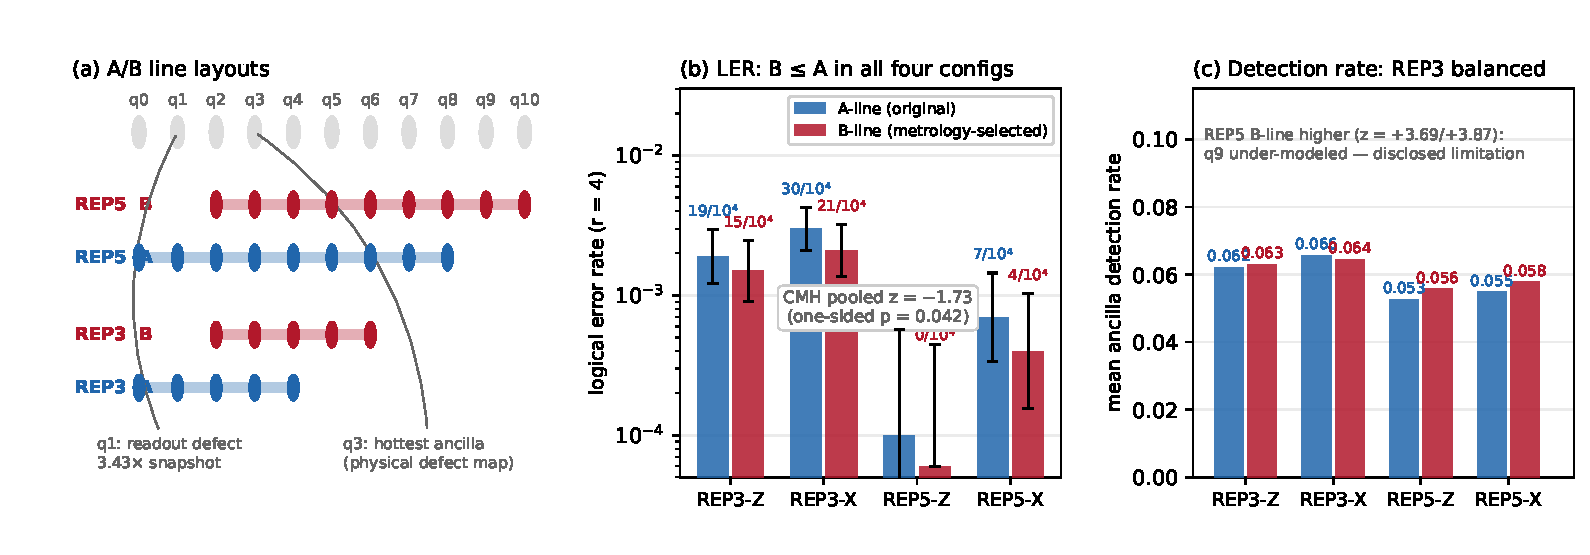
\includegraphics[width=\columnwidth]{figures/ap_f2_ab_result.pdf}
\caption{Active provenance: (a) A/B line layout with defect annotations;
  (b) logical error rates with Wilson CIs and the CMH pool;
  (c) per-detector event rates with the REP5 dissociation disclosed.}
\label{fig:ab}
\end{figure}

\section{Pre-registered device test of the injection-budget bound}
\label{app:injection}
%%-----------------------------------------------------------

We test Theorem~\ref{thm:spacetime} and Corollary~\ref{cor:stoch} on
ibm\_marrakesh (156-qubit Heron r2) with REP5 ($d{=}5$, $t{=}2$) and
REP3 ($d{=}3$, $t{=}1$) memories, both sectors, $R{=}4$ rounds.
The adversary injects Pauli faults at round~2 (Z-sector: physical $X$
gates; X-sector: basis-conjugated physical $X$ gates, H--$X$--H, realizing
$Z$-type faults on the $\lvert +_L \rangle$ memory; each injected fault is
thus implemented with native gates in both sectors). Layouts are the metrology-selected B-lines of
Appendix~\ref{app:activeprov}, fixed across all arms so that injection
is the only varying factor. Predictions, decision rules, seeds,
layouts, and circuit digests were pinned (SHA-256
\texttt{759169c2\dots c74653cd5}) \emph{before} submission; 312 arms
(180{,}000 shots) ran in four Sampler jobs
(\texttt{da8um21qtnsc73d0v3ug}, \texttt{da8um2ce74ec73aj4n3g},
\texttt{da8um31qtnsc73d0v400}, \texttt{da8um3ke74ec73aj4n50}); the full
noiseless pipeline was validated end-to-end (22/22 arms) before
submission. $\pi(k)$ entering the composed bounds is estimated from the
calibration-snapshot fault model ($\lambda_N{=}0.47$ faults/shot REP5,
$0.25$ REP3): $\pi(1..3)=0.375, 0.081, 0.012$ (REP5) and
$0.221, 0.027, 0.002$ (REP3). \textbf{Model status of $\pi$:} these
tails are \emph{predictions of a pinned model} --- a Poisson fault-count
law whose intensity $\lambda_N$ sums readout-error locations only
(gate/idle terms enter at second order on Heron r2). They are not
conservative envelopes over calibration drift; their empirical content
is tested by the arms below, not assumed. Scope: this campaign tests the
injection-budget bound and the calibration-to-model workflow on
repetition memories; it is not a measurement of BB-code hardware
performance, and no quantitative REP$\to$BB transfer is claimed.

\begin{table}[H]\centering\small
\caption{Deterministic worst-case injection arms (10{,}000 shots each).
``Bound'': Theorem~\ref{thm:spacetime}(c) with calibration $\pi$.}
\label{tab:injdet}
\begin{tabular}{@{}llrrrr@{}}
\toprule
arm & sector & failures & LER & bound & verdict \\\midrule
REP5 base & Z & 0 & 0.0000 & 0.012 & holds \\
REP5 base & X & 2 & 0.0002 & 0.012 & holds \\
REP5 $w{=}2$ worst & Z & 414 & 0.0414 & 0.375 & holds \\
REP5 $w{=}2$ worst & X & 506 & 0.0506 & 0.375 & holds \\
REP5 $w{=}3$ worst & Z & 9590 & 0.9590 & --- & sharp \\
REP5 $w{=}3$ worst & X & 9598 & 0.9598 & --- & sharp \\
REP3 base & Z & 14 & 0.0014 & 0.027 & holds \\
REP3 base & X & 28 & 0.0028 & 0.027 & holds \\
REP3 $w{=}1$ worst & Z & 276 & 0.0276 & 0.221 & holds \\
REP3 $w{=}1$ worst & X & 318 & 0.0318 & 0.221 & holds \\
REP3 $w{=}2$ worst & Z & 9292 & 0.9292 & --- & sharp \\
REP3 $w{=}2$ worst & X & 9240 & 0.9240 & --- & sharp \\\bottomrule
\end{tabular}
\end{table}

\begin{table}[H]\centering\small
\caption{Stochastic injection arms, REP5 (50 pinned variants $\times$ 200
shots per cell). ``Naive (pop.\ avg.)'': v23's independence-form
threshold $\delta_0+\Pr[\mathrm{Bin}\ge3]+\mathrm{tol}$. ``Naive
(mask-cond.)'': the mask-conditioned estimand, conditioning on the
realized pinned masks,
$\delta_0+\frac{1}{50}\sum_v\mathbf{1}[w(\mathrm{mask}_v)\ge
t{+}1]+\mathrm{tol}$ (\texttt{stoch\_reanalysis\_v24.csv}); the verdict
is read against this column. The conditioning estimand was adopted
retrospectively, at reanalysis after inspection of the realized masks
(Table~\ref{tab:chronology}). Composed: Corollary~\ref{cor:stoch} with
calibration $\pi$.}
\label{tab:injstoch}
\begin{tabular}{@{}llrrrrrl@{}}
\toprule
$p$ & sector & failures & LER & naive (pop.\ avg.) & naive
(mask-cond.) & composed & verdict \\\midrule
0.01 & Z & 1 & 0.0001 & 0.0024 & 0.0024 & 0.016 & holds \\
0.01 & X & 2 & 0.0002 & 0.0027 & 0.0027 & 0.016 & holds \\
0.05 & Z & 6 & 0.0006 & 0.0035 & 0.0024 & 0.035 & holds \\
0.05 & X & 9 & 0.0009 & 0.0039 & 0.0027 & 0.035 & holds \\
0.10 & Z & 211 & 0.0211 & 0.0109 & 0.0224 & 0.070 & holds \\
0.10 & X & 388 & 0.0388 & 0.0113 & 0.0427 & 0.070 & holds \\\bottomrule
\end{tabular}
\end{table}

Three findings. (i)~\emph{The distance cliff is real and sharp:}
weight-$t$ worst-case injections stay within the composed
correctability bound on both distances and both sectors, while
weight-$(t{+}1)$ injections collapse the memory at $92.4$--$96.0\%$
logical failure; the shortfall from $100\%$ is native-noise rescue of
order $\pi(1)$. (ii)~\emph{Injection amplifies native noise exactly as
the chain argument predicts:} the REP5 $w{=}2$ arms sit
$100$--$250\times$ above baseline but an order of magnitude inside the
composed bound --- the first quantitative measurement of
adversary--noise composition on a quantum memory.
(iii)~\emph{Stochastic arms and the correct estimand.} v23 reported the
$p{=}0.10$ cells as falsifying the independence-form stochastic bound
(Proposition~\ref{prop:stochastic}) at $2.1\times$ (Z) and $3.8\times$
(X). That verdict compared realized LER against the
\emph{population-averaged} threshold; the pinned protocol,
however, fixes 50 masks, so the correct threshold for the pinned
ensemble is
\emph{mask-conditioned} (an estimand correction adopted retrospectively,
after inspection --- Table~\ref{tab:chronology}): the X ensemble
realizes two weight-3 masks
versus $0.43$ expected under $\mathrm{Bin}(5,0.1)$ (realized tail
$0.04$), the Z ensemble one (tail $0.02$). Against the conditioned
thresholds ($0.0224$ Z, $0.0427$ X) the realized LERs ($0.0211$,
$0.0388$) do \emph{not} exceed, and the same holds for all six cells in
both campaigns (\texttt{stoch\_reanalysis\_v24.csv}, 12 cells, margins
$0.0013$--$0.0039$): \textbf{the falsification verdict is withdrawn}.
What survives is a genuine observation --- the population-average form
undershoots realized-mask risk whenever the realized ensemble is
tail-heavy --- which \emph{motivated} the composed
Binomial$\otimes$Poisson model (Corollary~\ref{cor:stoch}) as a
discovery. That model is therefore reported as discovery, not as a
pre-registered prediction; its confirmatory test is the consolidation
campaign of Appendix~\ref{app:injection-repl}. The device-aware composed
form holds on all six stochastic arms and all eight bounded
deterministic arms under either estimand.

\paragraph{Security corollary.}
Combined with the REP5 detection-rate dissociation of
Appendix~\ref{app:activeprov} (placement moves the detection rate, not
the logical rate), these results imply that syndrome-level statistics
cannot certify memory integrity: a memory is certifiably
$(W,\eta)$-integrity-secure --- $\lambda_{\mathcal{M}}(W)\le\eta$ under
$\mathfrak{A}_1^{\mathrm{st}}(W)$ --- only via logical-level injection
probing of the kind reported here.

\subsection{Replication: second calibration cycle, second device,
distance~7}\label{app:injection-repl}

A pre-registered consolidation campaign (predictions, decision rules,
seeds, layouts, estimator, and digests pinned before submission, SHA-256
\texttt{cef236ce\dots de53aa1}) re-ran the test on
ibm\_marrakesh on a second calibration cycle (2026-09-06; 240{,}000
shots in four Sampler jobs \texttt{daelek5nj4cs73afaqpg},
\texttt{daelekd1ierc738mai50}, \texttt{daelel642tqs73auss4g},
\texttt{daeleljdd5gc73d8pcrg}), extended it to REP7 ($d{=}7$, $t{=}3$;
worst-case central strings $w{=}3$ and $w{=}4$), and replicated the REP5
deterministic arms on a second device, ibm\_fez (60{,}000 shots; jobs
\texttt{daelelt1ierc738mai7g}, \texttt{daelembdd5gc73d8pct0}). Layouts
were re-selected from the pinned 2026-09-06 snapshots by the
metrology rule of Appendix~\ref{app:activeprov} (the REP5 rule returned
the campaign-1 line); the stochastic masks are bit-identical to
campaign~1. The native-fault estimator is pinned explicitly,
$\lambda_N=\sum_{\mathrm{data}}\epsilon_{\mathrm{ro}}+
R\sum_{\mathrm{anc}}\epsilon_{\mathrm{ro}}$ with symmetric readout
$\epsilon_{\mathrm{ro}}$ (readout locations dominate the Heron-r2
spacetime budget; gate/idle terms are second order): $\lambda_N{=}0.088,
0.222, 0.347$ (REP3/5/7, marrakesh) and $0.453$ (REP5, fez) --- the
2026-09-06 marrakesh calibration is substantially cleaner than that of
2026-08-28 ($\lambda_N{=}0.25, 0.47$). Noiseless end-to-end validation
passed on all 42 checked arms before submission.

\begin{table}[H]\centering\small
\caption{Consolidation deterministic arms (10{,}000 shots each): REP7
extension (ibm\_marrakesh) and second-device REP5 replication
(ibm\_fez). ``Bound'': Theorem~\ref{thm:spacetime}(c) with the pinned
calibration $\pi$.}
\label{tab:injrepl}
\begin{tabular}{@{}lllrrrl@{}}
\toprule
device & arm & sector & failures & LER & bound & verdict \\\midrule
marrakesh & REP7 base & Z & 0 & 0.0000 & 0.0005 & holds \\
 & REP7 $w{=}3$ worst & Z & 568 & 0.0568 & 0.293 & holds \\
 & REP7 $w{=}4$ worst & Z & 9691 & 0.9691 & --- & sharp \\
 & REP7 base & X & 1 & 0.0001 & 0.0005 & holds \\
 & REP7 $w{=}3$ worst & X & 675 & 0.0675 & 0.293 & holds \\
 & REP7 $w{=}4$ worst & X & 9599 & 0.9599 & --- & sharp \\\midrule
fez & REP5 base & Z & 1 & 0.0001 & 0.011 & holds \\
 & REP5 $w{=}2$ worst & Z & 484 & 0.0484 & 0.364 & holds \\
 & REP5 $w{=}3$ worst & Z & 9768 & 0.9768 & --- & sharp \\
 & REP5 base & X & 6 & 0.0006 & 0.011 & holds \\
 & REP5 $w{=}2$ worst & X & 683 & 0.0683 & 0.364 & holds \\
 & REP5 $w{=}3$ worst & X & 9745 & 0.9745 & --- & sharp \\\bottomrule
\end{tabular}
\end{table}

Four findings. (i)~\emph{Full replication.} On the new calibration cycle
every campaign-1 verdict reproduces: all bounded deterministic arms sit
$4$--$8\times$ inside the composed bound on both distances and sectors
(REP3 $w{=}1$: $0.0102/0.0202$ vs bound $0.084$; REP5 $w{=}2$:
$0.0333/0.0436$ vs $0.199$), all weight-$(t{+}1)$ arms remain sharp
($0.898$--$0.974$), and all six stochastic cells track campaign~1 within
statistical noise (at $p{=}0.10$: $0.0202$ vs $0.0211$ Z; $0.0403$ vs
$0.0388$ X). The campaign-1 excess over the population-averaged
independence-form threshold replicates ($1.9\times$ Z, $3.6\times$ X),
and, as in campaign~1, no cell exceeds the mask-conditioned threshold
($0.0224$ Z, $0.0426$ X) --- for this consolidation the estimand was
part of the pre-submission pinning, so no falsification
occurs in either campaign under the correct estimand
(\texttt{stoch\_reanalysis\_v24.csv}).
(ii)~\emph{The cliff has a third distance point.} REP7 behaves as
Theorem~\ref{thm:spacetime} demands: weight-$3$ worst-case injections
stay inside the bound ($0.057/0.068$ vs $0.293$) while weight-$4$
collapses the memory at $96.0$--$96.9\%$; the cliff is sharp at
$d{=}3,5,7$. (iii)~\emph{Cross-device.} The REP5 pattern reproduces on
ibm\_fez with its own pinned calibration ($\lambda_N{=}0.453$): bounds
hold at $5$--$7\times$ margin, sharpness at $97.5$--$97.7\%$.
(iv)~\emph{Mask-level composition.} With the cleaner calibration the
population-average binomial-form composed bound tightens ($0.0335$ for
the X-sector $p{=}0.10$ cell), and the realized LER ($0.0403$) exceeds
that population-average form by $1.20\times$; the excess is entirely
accounted for by the realized pinned-mask ensemble --- the X masks
contain two weight-3 variants versus $0.43$ expected under
$\mathrm{Bin}(5,0.1)$, contributing $0.0375$ --- and conditioning the
composed bound on the realized masks (bound $0.0665$) restores it: the
composition law holds mask-by-mask, not only in binomial expectation.
This is the same estimand correction as in campaign~1, applied to the
composed model. Absolute LERs of bounded
arms drift down coherently with the cleaner calibration
($\lambda_N$: $0.47{\to}0.22$), while cliff arms drift slightly up (less
native-noise rescue of order $\pi(1)$), exactly as the model predicts.
The consolidation artifacts (\texttt{theory\_test\_consol/}) are archived
with the same digest discipline as campaign~1.

%%-----------------------------------------------------------
\section{Chronology and protocol-pinning ledger}\label{app:chronology}
%%-----------------------------------------------------------

Table~\ref{tab:chronology} records, for every campaign in this work,
what was frozen before data-taking and what was amended after
inspection. Terminology: \emph{pinned} means the artifact (protocol,
masks, seeds, predictions, decision rules, digests) was hash-frozen
before the corresponding runs; \emph{retrospective} means the estimand
or rule was adopted after inspecting data. Nothing in this manuscript is
described as pre-registered beyond the pinnings listed here, and every
estimand adopted after data inspection is labeled retrospective both
here and at its point of use.

\begin{table}[H]\centering\scriptsize
\caption{Chronology ledger: date, campaign, what was frozen before
  data-taking, estimand status, result, and amendments. Hashes are
  SHA-256 prefixes of the pinned prediction bundles.}
\label{tab:chronology}
\setlength{\tabcolsep}{4pt}
\begin{tabular}{@{}p{1.4cm}p{2.7cm}p{3.8cm}p{3.2cm}p{3.4cm}@{}}
\toprule
date & campaign & frozen before data-taking & estimand status &
result / amendments \\\midrule
2026-08-28 & placement A/B pilot
  (App.~\ref{app:activeprov})
  & line-selection rule and A/B pairing from the 2026-08-28 snapshot
    (\texttt{MANIFEST.json} 08:28~UTC) before the 40-minute run window
  & paired-LFR association (CMH), exploratory
  & 4/4 configurations favor B-lines; pooled $p{=}0.042$, exact
    stratified $p{=}0.0517$; reported as descriptive pilot, no causal
    claim \\\addlinespace
2026-08-28 & device campaign~1
  (App.~\ref{app:injection})
  & predictions, decision rules, seeds, layouts, circuit digests
    hash-pinned (\texttt{759169c2\dots}); 22/22 noiseless validation
    passed pre-submission
  & pinned estimand: population-averaged thresholds and deterministic
    bound verdicts
  & deterministic bounds hold; weight-$(t{+}1)$ sharp; stochastic
    $p{=}0.10$ cells exceed the pinned threshold $2.1$--$3.8\times$
    (verdict later withdrawn --- next row) \\\addlinespace
2026-09 & campaign-1 reanalysis (amendment)
  & --- (analysis-only; no new device data)
  & mask-conditioned estimand adopted \emph{retrospectively}, after
    inspection of the realized masks
  & falsification verdict withdrawn; composed Binomial$\otimes$Poisson
    model developed as \emph{discovery}; not part of the pre-submission
    pinning \\\addlinespace
2026-09-06 & consolidation
  (App.~\ref{app:injection-repl})
  & predictions, rules, seeds, layouts, estimator, digests hash-pinned
    (\texttt{cef236ce\dots}); stochastic masks bit-identical to
    campaign~1
  & mask-conditioned estimand \emph{included} in the pre-submission
    pinning (carried over from the campaign-1 correction)
  & full replication on a second calibration cycle; REP7 ($d{=}7$)
    extension; second-device (ibm\_fez) replication \\\addlinespace
v23 cycle & comparator grid; repeated-cycle fixed ladder
  & paired streams and grid frozen per archived run manifests
  & exploratory; $\pm0.5\%$ equivalence margin adopted retrospectively
    for the archived grid (pinned only for the confirmatory protocol)
  & archived as exploratory; equivalence statements are at-margin, not
    point-null \\\addlinespace
v24 freeze & injection-boundary decoders; adaptive RC extension
  & frozen probe set and frozen native-error replay
    (\texttt{ibd\_v24\_freeze.json}); adaptive stopping rule pinned
    before launch
  & four-category endpoint; adaptive arms analysed with time-uniform
    confidence sequences
  & second-round-review repairs (2026-09): worst-case interval rule
    corrected (Remark~\ref{rem:intervals}); adaptive intervals
    regenerated with Robbins mixture sequences
    (\texttt{stats\_intervals.py}); endpoint classifier made
    true-residual-based with a regression test
    (App.~\ref{app:injection} endpoint audit) \\\addlinespace
2026-09 & WS-C circuit arm (Sec.~\ref{sec:circuit})
  & corrected extraction circuit (C01 repair) with invariance checks;
    six-rate grid pinned per-point with checkpointing
  & fixed-$N$ arms, Wilson/CP per arm
  & single corrected point archived; the full corrected grid is
    regenerated from the pinned per-point runners and merged into
    Table~\ref{tab:wsc} \\\bottomrule
\end{tabular}
\end{table}

\emph{Standing consequence.} Any future amendment enters this ledger
with its date and pinning status; claims whose estimands are
retrospective (the placement pilot, the campaign-1 mask conditioning,
the archived-grid equivalence margin) are excluded from any
confirmatory reading of this work.

%%-----------------------------------------------------------
\section{Illustrative routing arithmetic}\label{app:routing}
\emph{Heuristic only; LFR underestimates diamond-norm error.}
$J=8$, $b=1$, $\Delta=0.05$: $p_\mathrm{hit}\le0.175$.
CZ at $p=5\times10^{-4}$: $(0.825)(0.905)=0.747$.
MS: $(0.825)(0.955)=0.788$.

\bibliographystyle{unsrtnat}
\bibliography{references}
\end{document}
